%%%%%%%%%%%%%%%%%%%%%%%%%
%% Header for standard beamer presentation
%%
%%  PresentationHeader.tex
%%
%%%%%%%%%%%%%%%%%%%%%%%%%

\documentclass[english,10pt]{beamer}

%%%%%%%%%%%%%%%%%%%%
%% Include general header where common packages are defined
%%%%%%%%%%%%%%%%%%%%



%%%%%%%%%%%%%%%%%%%%%%%%%%
%% TEMPLATES
%%%%%%%%%%%%%%%%%%%%%%%%%%


% Simple Tabular

%\begin{tabular}{ |c|c|c| } 
% \hline
% cell1 & cell2 & cell3 \\ 
% cell4 & cell5 & cell6 \\ 
% cell7 & cell8 & cell9 \\ 
% \hline
%\end{tabular}





%%%%%%%%%%%%%%%%%%%%%%%%%%
%% Packages
%%%%%%%%%%%%%%%%%%%%%%%%%%


% general packages without options
\usepackage{amsmath,amssymb,amsthm,bbm}

% graphics
\usepackage{graphicx,transparent,eso-pic}

% text formatting
\usepackage[document]{ragged2e}
\usepackage{pagecolor,color,ulem,soul}








%%%%%%%%%%%%%%%%%%%%%%%%%%
%% Maths environment
%%%%%%%%%%%%%%%%%%%%%%%%%%

%\newtheorem{theorem}{Theorem}[section]
%\newtheorem{lemma}[theorem]{Lemma}
%\newtheorem{proposition}[theorem]{Proposition}
%\newtheorem{corollary}[theorem]{Corollary}

%\newenvironment{proof}[1][Proof]{\begin{trivlist}
%\item[\hskip \labelsep {\bfseries #1}]}{\end{trivlist}}
%\newenvironment{definition}[1][Definition]{\begin{trivlist}
%\item[\hskip \labelsep {\bfseries #1}]}{\end{trivlist}}
%\newenvironment{example}[1][Example]{\begin{trivlist}
%\item[\hskip \labelsep {\bfseries #1}]}{\end{trivlist}}
%\newenvironment{remark}[1][Remark]{\begin{trivlist}
%\item[\hskip \labelsep {\bfseries #1}]}{\end{trivlist}}

%\newcommand{\qed}{\nobreak \ifvmode \relax \else
%      \ifdim\lastskip<1.5em \hskip-\lastskip
%      \hskip1.5em plus0em minus0.5em \fi \nobreak
%      \vrule height0.75em width0.5em depth0.25em\fi}



%%%%%%%%%%%%%%%%%%%%
%% Idem general commands
%%%%%%%%%%%%%%%%%%%%

%\input{/Users/Juste/Documents/ComplexSystems/CityNetwork/Docs/Headers/GeneralCommands.tex}


\usetheme{Boadilla}

%\setbeamertemplate{footline}[text line]{}
%\setbeamercolor{structure}{fg=purple!50!blue, bg=purple!50!blue}

% cybergeo palette (from Clem server)
% #1C6F91, "#df691a", "#77c5ba", "orange", "#2db92d", "#e1ff2f", "#ff2313", "#bbab61
% redefine palette
\definecolor{cybblue}{HTML}{1C6F91}
\definecolor{cyborange}{HTML}{DF691A}
\definecolor{cybbluegreen}{HTML}{77C5BA}
\definecolor{cybgreen}{HTML}{2DB92D}
\definecolor{cybgreenyellow}{HTML}{E1FF2F}
\definecolor{cybred}{HTML}{FF2313}
\definecolor{cybglaucous}{HTML}{BBAB61}


\setbeamercolor{structure}{fg=cybblue}
\setbeamercolor{footline}{fg=orange, bg=orange}

\setbeamercovered{transparent}


\addtobeamertemplate{title page}{\hspace{-0.4cm}\vspace{-1.5cm}\includegraphics[height=1.2cm,width=1.2\textwidth]{template/bandeau3}\\
}{%
%\begin{textblock*}{150mm}(-1cm,-1.5cm)
%\end{textblock*}
}




\addtobeamertemplate{frametitle}{\hspace{-0.4cm}\vspace{-0.1cm}\includegraphics[height=1.2cm,width=1.2\textwidth]{template/bandeau3}\\
}{%
%\begin{textblock*}{150mm}(-1cm,-1.5cm)
%\end{textblock*}
}



% shortened command for a justified frame
\newcommand{\jframe}[2]{\frame{\frametitle{#1}\justify{#2}}}


\newcommand{\noun}[1]{\textsc{#1}}
\newcommand{\jitem}[1]{\item \begin{justify} #1 \end{justify} \vfill{}}
\newcommand{\sframe}[2]{\frame{\frametitle{#1} #2}}

\DeclareMathOperator{\Cov}{Cov}
\DeclareMathOperator{\Var}{Var}
\DeclareMathOperator{\E}{\mathbb{E}}
\DeclareMathOperator{\Proba}{\mathbb{P}}

\newcommand{\Covb}[2]{\ensuremath{\Cov\!\left[#1,#2\right]}}
\newcommand{\Eb}[1]{\ensuremath{\E\!\left[#1\right]}}
\newcommand{\Pb}[1]{\ensuremath{\Proba\!\left[#1\right]}}
\newcommand{\Varb}[1]{\ensuremath{\Var\!\left[#1\right]}}

% norm
\newcommand{\norm}[1]{\| #1 \|}

\newcommand{\indep}{\rotatebox[origin=c]{90}{$\models$}}


\usepackage{textpos}



%%%%%%%%%%%%%%%%%%%%%
%% Begin doc
%%%%%%%%%%%%%%%%%%%%%

\begin{document}


\title{Indirect Bibliometrics by Complex Network Analysis}


\author{J.~Raimbault$^{1,2}$}

%\authorrunning{J.~Raimbault}

\institute{$^{1}$G{\'e}ographie-cit{\'e}s (UMR 8504 CNRS)\\
$^{2}$LVMT (UMR-T 9403 IFSTTAR)}

\date{Cybergeo : 20 ans d{\'e}j{\`a} !\\
Jeudi 26 mai 2016}

%
%\usebackgroundtemplate{%
%  \AddToShipoutPicture*{
%    \put(0,0){
%        \parbox[b][\paperheight]{\paperwidth}{%
%            \vfill
%            \centering
%            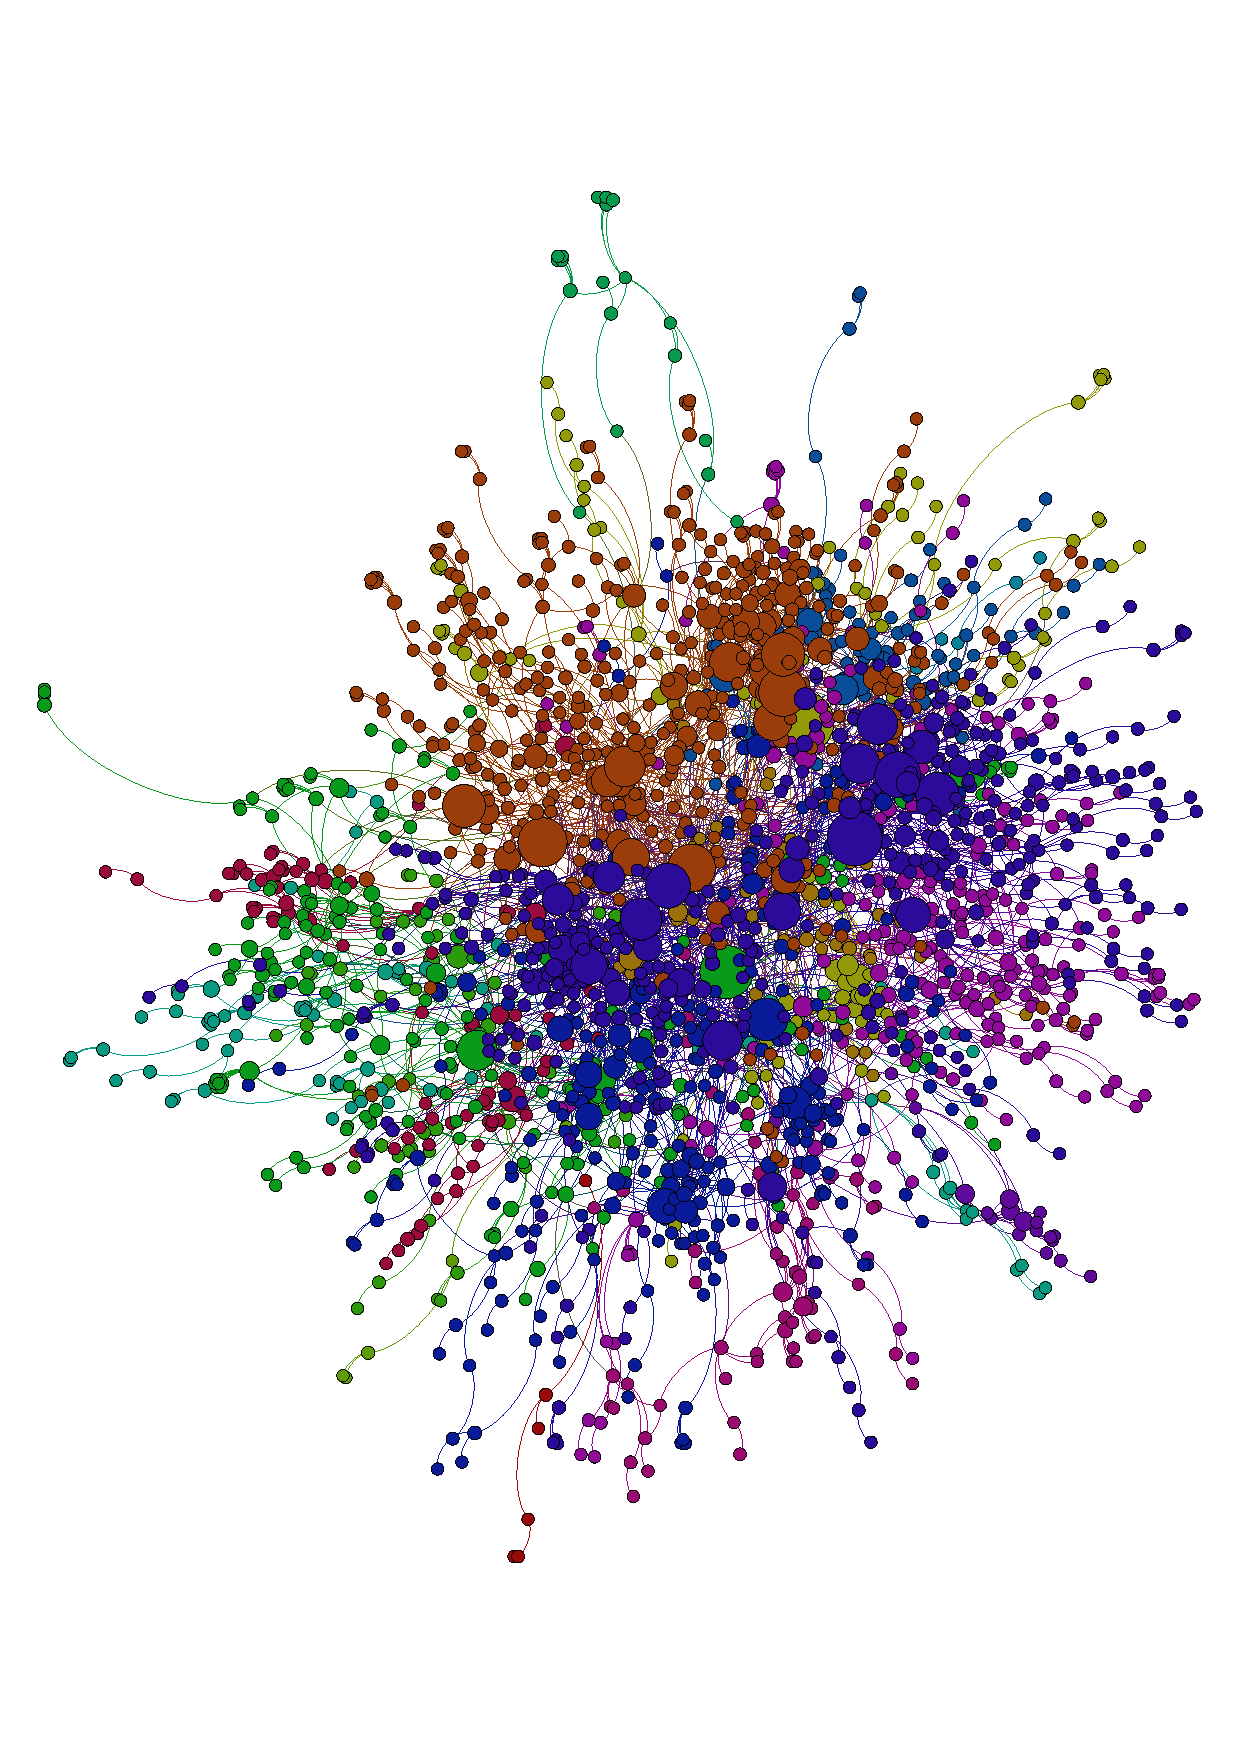
\includegraphics[width=\paperwidth]{figures/nw}%
%            \vfill
%        }
%    }
%    \put(0,0){%
%        \transparent{0.9}\textcolor{white}{\rule{\paperwidth}{\paperheight}}
%    }
%}
%  %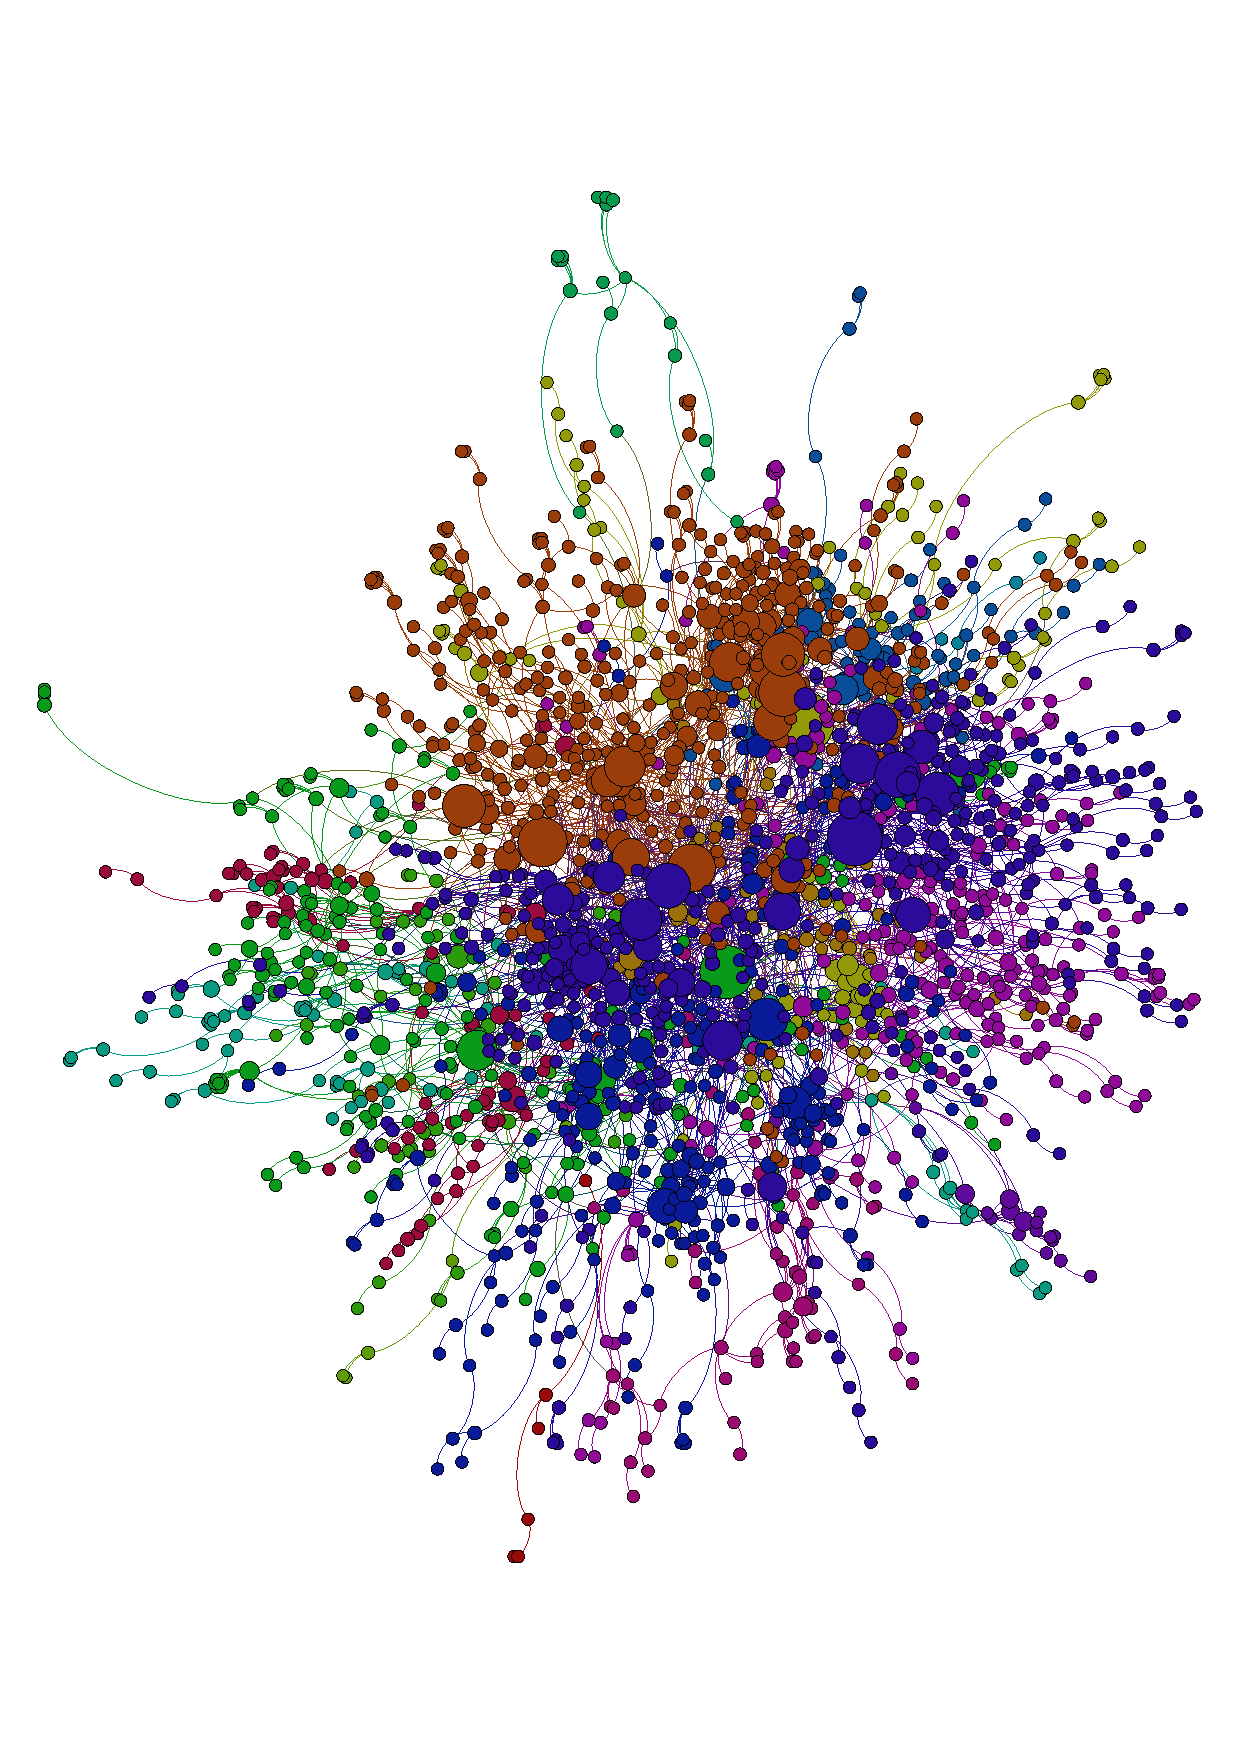
\includegraphics[width=1.5\paperwidth,height=1.5\paperheight]{figures/nw}
%} 






%%%%%%%%%%%%%%%%%%%%%%%%%%%%%%%%
\begin{frame}
\titlepage
\end{frame}

% NO TOC
%\begin{frame}
%\tableofcontents
%\end{frame}
%%%%%%%%%%%%%%%%%%%%%%%%%%%%%%%%


\usebackgroundtemplate{}


\section{Introduction}



\jframe{Context}{

%\textit{``You are what you cite''} : \textbf{Quels sont les environnements disciplinaires voisins de Cybergeo ? Sont-ils différents des contenus des articles (POC) et des contenus d{\'e}clar{\'e}s (HC) ?}

\textit{``You are what you cite''} : \textbf{Which disciplines populate the scientific neighborhood of cybergeo ? Are they different from the ones obtained through article content (POC) and declared contents (HC)  analysis ?}



\bigskip

%$\rightarrow$ Enjeu par rapport {\`a} la ligne {\'e}ditoriale de la revue : interdisciplinarit{\'e} et ouverture

$\rightarrow$ Important for editorial policy : interdisciplinarity and Open Science

\bigskip

$\rightarrow$ Semi-qualitative approach, against a purely quantitative bibliometric harmful to humanities

\bigskip

}

\jframe{Objective}{

%\textbf{Question de recherche : }\textit{Dans quelle mesure le croisement d'une approche par r{\'e}seau de citation avec une approche par analyse s{\'e}mantique peut-il permettre d'analyser le contexte disciplinaire de la revue ?}

\textbf{Research question : }\textit{How does the combination of a citation network approach with a semantic analysis unveil disciplinary context of the journal ?}

\bigskip

%$\rightarrow$ Elaboration d'une m{\'e}thodologie d'analyse d'\textit{Hyperr{\'e}seau} : croisement d'un r{\'e}seau de citations {\`a} un r{\'e}seau s{\'e}mantique. Gain d'information par croisement des couches (d{\'e}marche transversale) %analogie avec construction scientifique : cf CS Roadmap)

$\rightarrow$ Hypernetwork methodology : superposition of a citation network with a semantic network, in the spirit of a transversal approach

\bigskip

%$\rightarrow$ Donn{\'e}es difficiles d'acc{\`e}s : base {\`a} construire
 
$\rightarrow$ Data difficult to access : database to construct


}



\section{Data collection}



\jframe{Data collection}{

\textbf{Cybergeo data} : journal production base

\medskip

$\rightarrow$ Structuration and Consolidation

\bigskip

\textbf{Citation data} : cybergeo not indexed 

\medskip

%$\rightarrow$ \textit{crawling} de \texttt{google scholar} par utilisation de l'option ``\textit{cit{\'e} par}'' \cite{noruzi2005google}

$\rightarrow$ \texttt{google scholar} crawling by using ``\textit{cited by}'' option\cite{noruzi2005google}

\bigskip

%\textbf{Donn{\'e}es textuelles} : besoin des r{\'e}sum{\'e}s pour l'ensemble des r{\'e}f{\'e}rences li{\'e}es 

\textbf{Text data} : need abstracts for all linked articles

\medskip

%$\rightarrow$ utilisation de l'API Mendeley~\cite{mendeley} (gratuite mais non ouverte).

$\rightarrow$ use of Mendeley API~\cite{mendeley} (free but not open)

}


\jframe{Data Collection Architecture}{
\includegraphics[height=0.76\textheight]{figures/archi}
}





\section{Methods and Results}

\subsection{Citation Network}


\jframe{Network Properties}{


$\rightarrow$ $\simeq$ 947 cybergeo articles can be studied, among $\simeq 1200$

\smallskip

$\rightarrow$ \textit{418670 Nodes et 570352 Links ; Diameter : 9 ; Density : 3.25E-6 ; average degree : 2.724284}

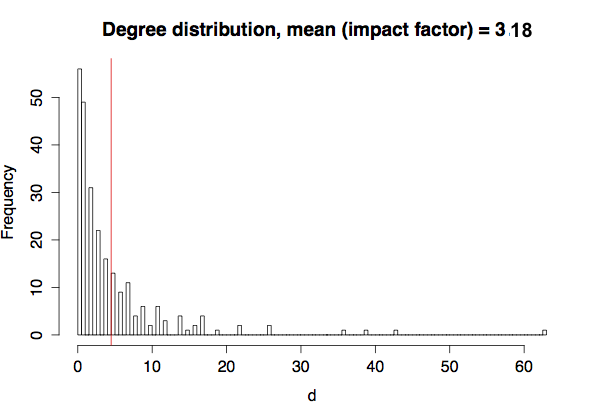
\includegraphics[width=0.75\textwidth]{figures/degreeDistrib.png}
}


\jframe{Citation Network Structure}{
\includegraphics[height=0.75\textheight]{figures/citnw}
}




\jframe{Degr{\'e}s : Loi rang-taille}{
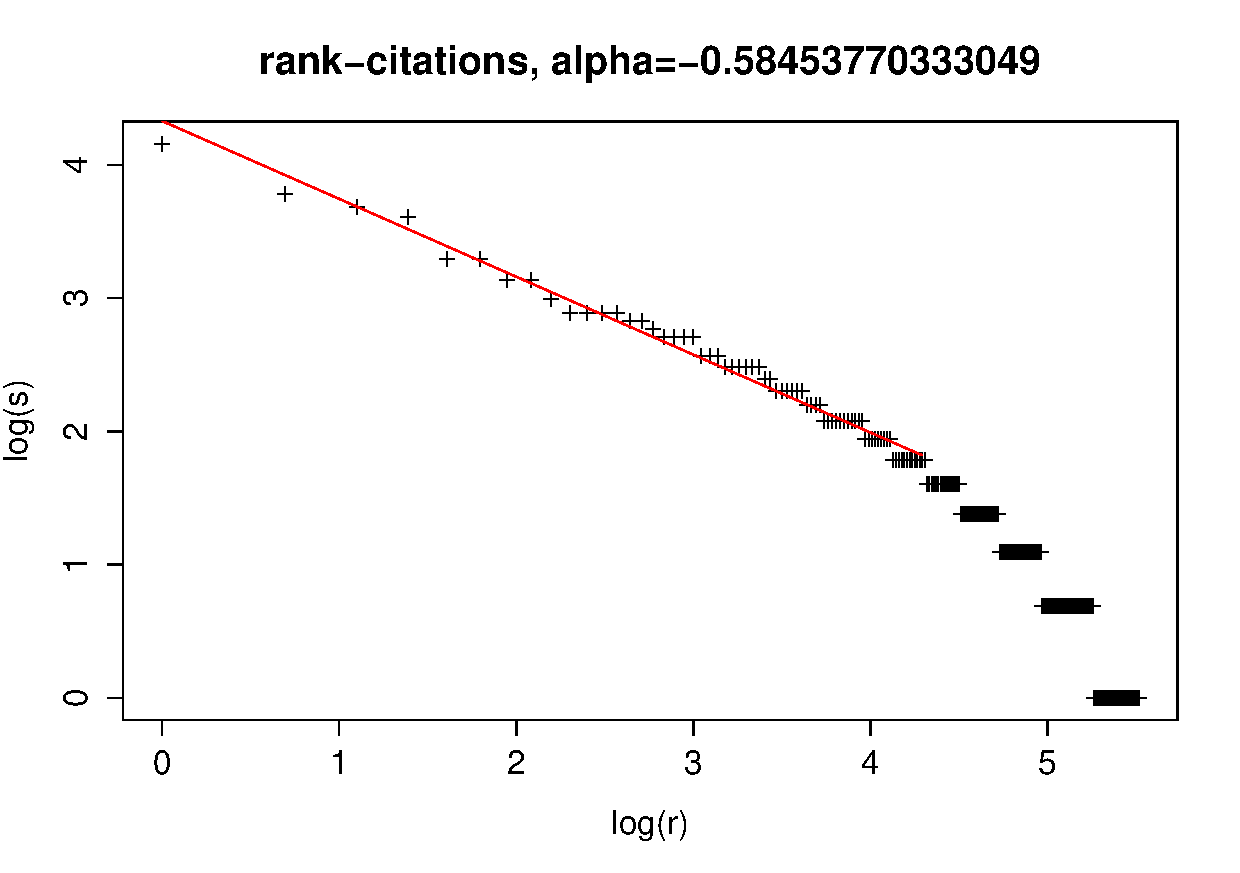
\includegraphics[width=0.52\textwidth]{figures/rankSize_fit}
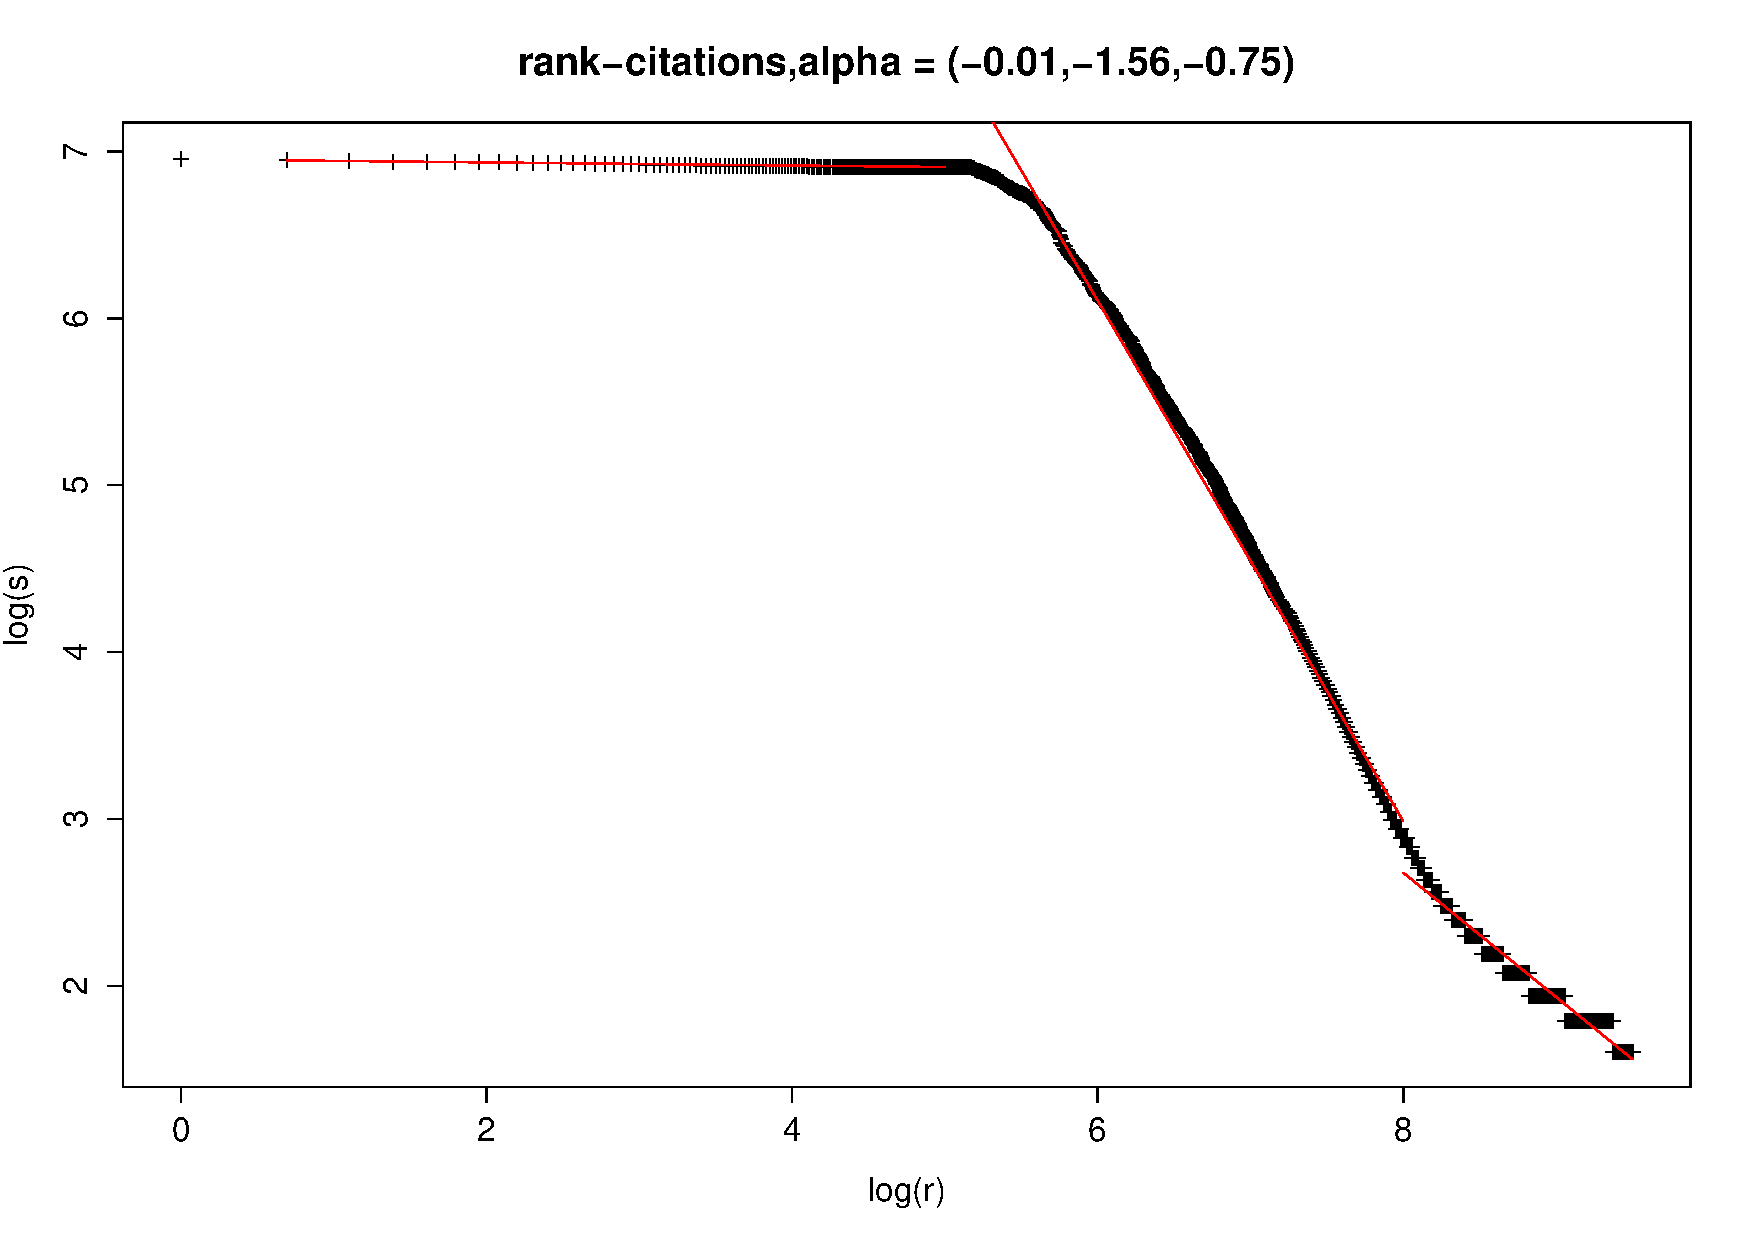
\includegraphics[width=0.5\textwidth]{figures/rank-size-all}

\textit{Gauche : Cyberg{\'e}o ; Droite : Ensemble du r{\'e}seau}

}




\jframe{Cliques}{
\vspace{-1cm}
\hspace{-2.3cm}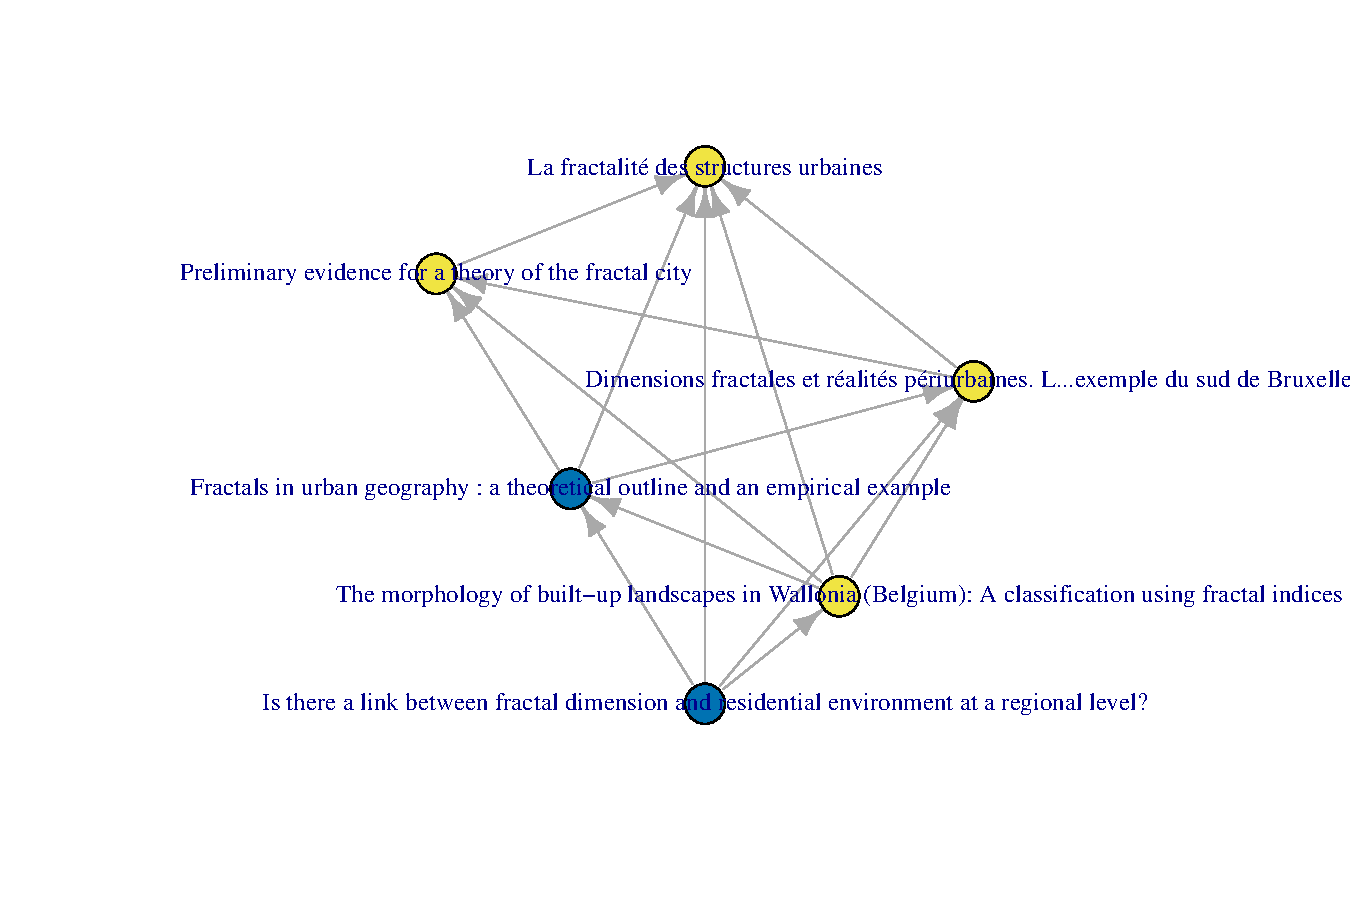
\includegraphics[height=\textheight]{figures/cybclic_2cyb_13761}

}







\subsection{Semantic Network}


\jframe{R{\'e}seau s{\'e}mantique}{


\textbf{R{\'e}seau s{\'e}mantique.} Collection des r{\'e}sum{\'e}s/ann{\'e}es/auteurs/mots-cl{\'e}s pour les 400000 r{\'e}f{\'e}rences via l'API Mendeley
$\rightarrow$ $\sim 215000$ r{\'e}f{\'e}rences avec donn{\'e}es compl{\`e}tes.

\bigskip

\textbf{Statistiques}

\textit{Langues :} anglais 206607, francais 4109, espagnol 2029, allemand 892, portugais 891, n{\'e}erlandais 124, autres 182

\textit{Repartitions par ann{\'e}es : }
\centering

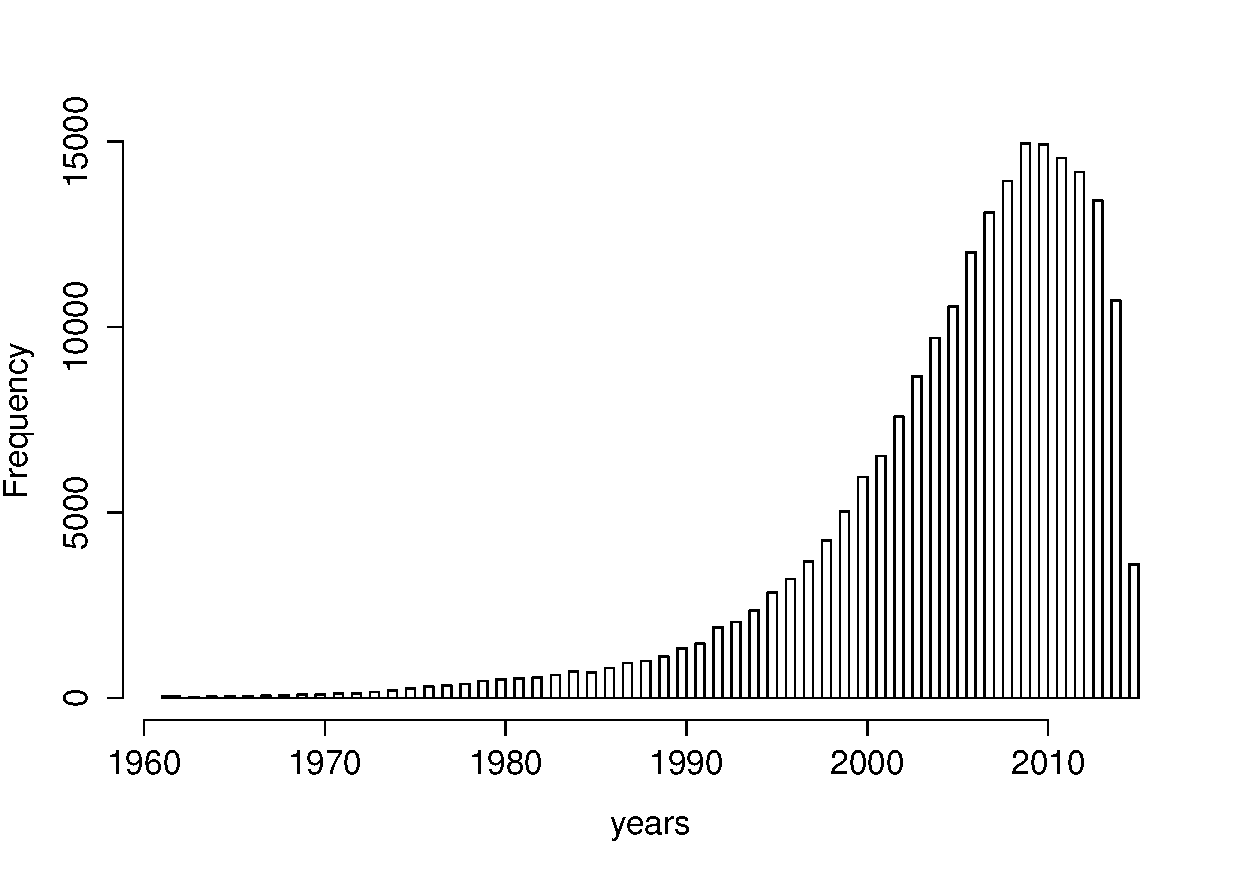
\includegraphics[width=0.4\textwidth,height=0.4\textheight]{figures/years}

}



\jframe{Keywords Extraction}{

%\textit{Text-mining en python avec \texttt{nltk}~\cite{bird2006nltk}}, m{\'e}thode adapt{\'e}e de
%\cite{chavalarias2013phylomemetic}

\textit{Text-mining in python with \texttt{nltk}~\cite{bird2006nltk}}, method adpated from
\cite{chavalarias2013phylomemetic}

%\begin{itemize}
%\item Detection de la langue par \textit{stop-words} (mots vides de sens)
%\item Parsing et tokenizing (isolation des mots) /pos-tagging (fonction des mots) /stemming (extraction de la racine) effectu{\'e}s diff{\'e}remment selon la langue :
%\begin{itemize}
%\item Anglais : pos-tagger int{\'e}gr{\'e} {\`a} \texttt{nltk}, combin{\'e} {\`a} un \emph{PorterStemmer}
%\item Fran\c{c}ais ou autre : utilisation de \texttt{TreeTagger}~\cite{schmid1994probabilistic}
%\end{itemize}
%\item Selection des \textit{n-grams} potentiels (avec $1 \leq n \leq 4$) : anglais $\bigcap \{NN \cup VBG \cup JJ \}$ ;  français  $\bigcap \{NOM \cup ADJ\}$
%\item Insertion en base pour extraction quasi-instantanée plus tard (10j $\rightarrow$ 5min)
%\item Estimation de la pertinence des \textit{n-grams} selon r{\'e}partition statistique des co-occurrences
%\end{itemize}

\begin{itemize}
\item Language detection using \textit{stop-words}
\item Parsing and tokenizing / pos-tagging (word functions) / stemming done differently depending on language :
\begin{itemize}
\item English : \texttt{nltk} built-in pos-tagger, combined to a \emph{PorterStemmer}
\item French or other : use of \texttt{TreeTagger}~\cite{schmid1994probabilistic}
\end{itemize}
\item Selection of potential \textit{n-grams} (with $1 \leq n \leq 4$) : English $\bigcap \{NN \cup VBG \cup JJ \}$ ;  French  $\bigcap \{NOM \cup ADJ\}$
\item Database insertion for instantaneous utilisation (10j $\rightarrow$ 2min)
\item Estimation of \textit{n-grams} relevance, following co-occurrences statistical distribution
\end{itemize}


}




\jframe{Construction of Semantic Network}{

\begin{itemize}

\item \textbf{Noeuds :} Mots-cl{\'e}s avec la plus grande pertinence cumul{\'e}e

\medskip

\item \textbf{Liens :} Co-occurrences pond{\'e}r{\'e}es

\medskip

\item Filtrage des liens en dessous d'un seuil ; ajustement manuel de mots parasites

\medskip

\item Detection de communaut{\'e}s par maximisation de modularit{\'e} \cite{blondel2008fast} apr{\`e}s suppression des \textit{hubs} (ex. \texttt{model}, \texttt{space}, \texttt{structure}, \texttt{process})

\end{itemize}

%Spatialisation de \textit{Fruchterman-Reingold}

}



%\jframe{R{\'e}seau s{\'e}mantique : r{\'e}seau brut}{
%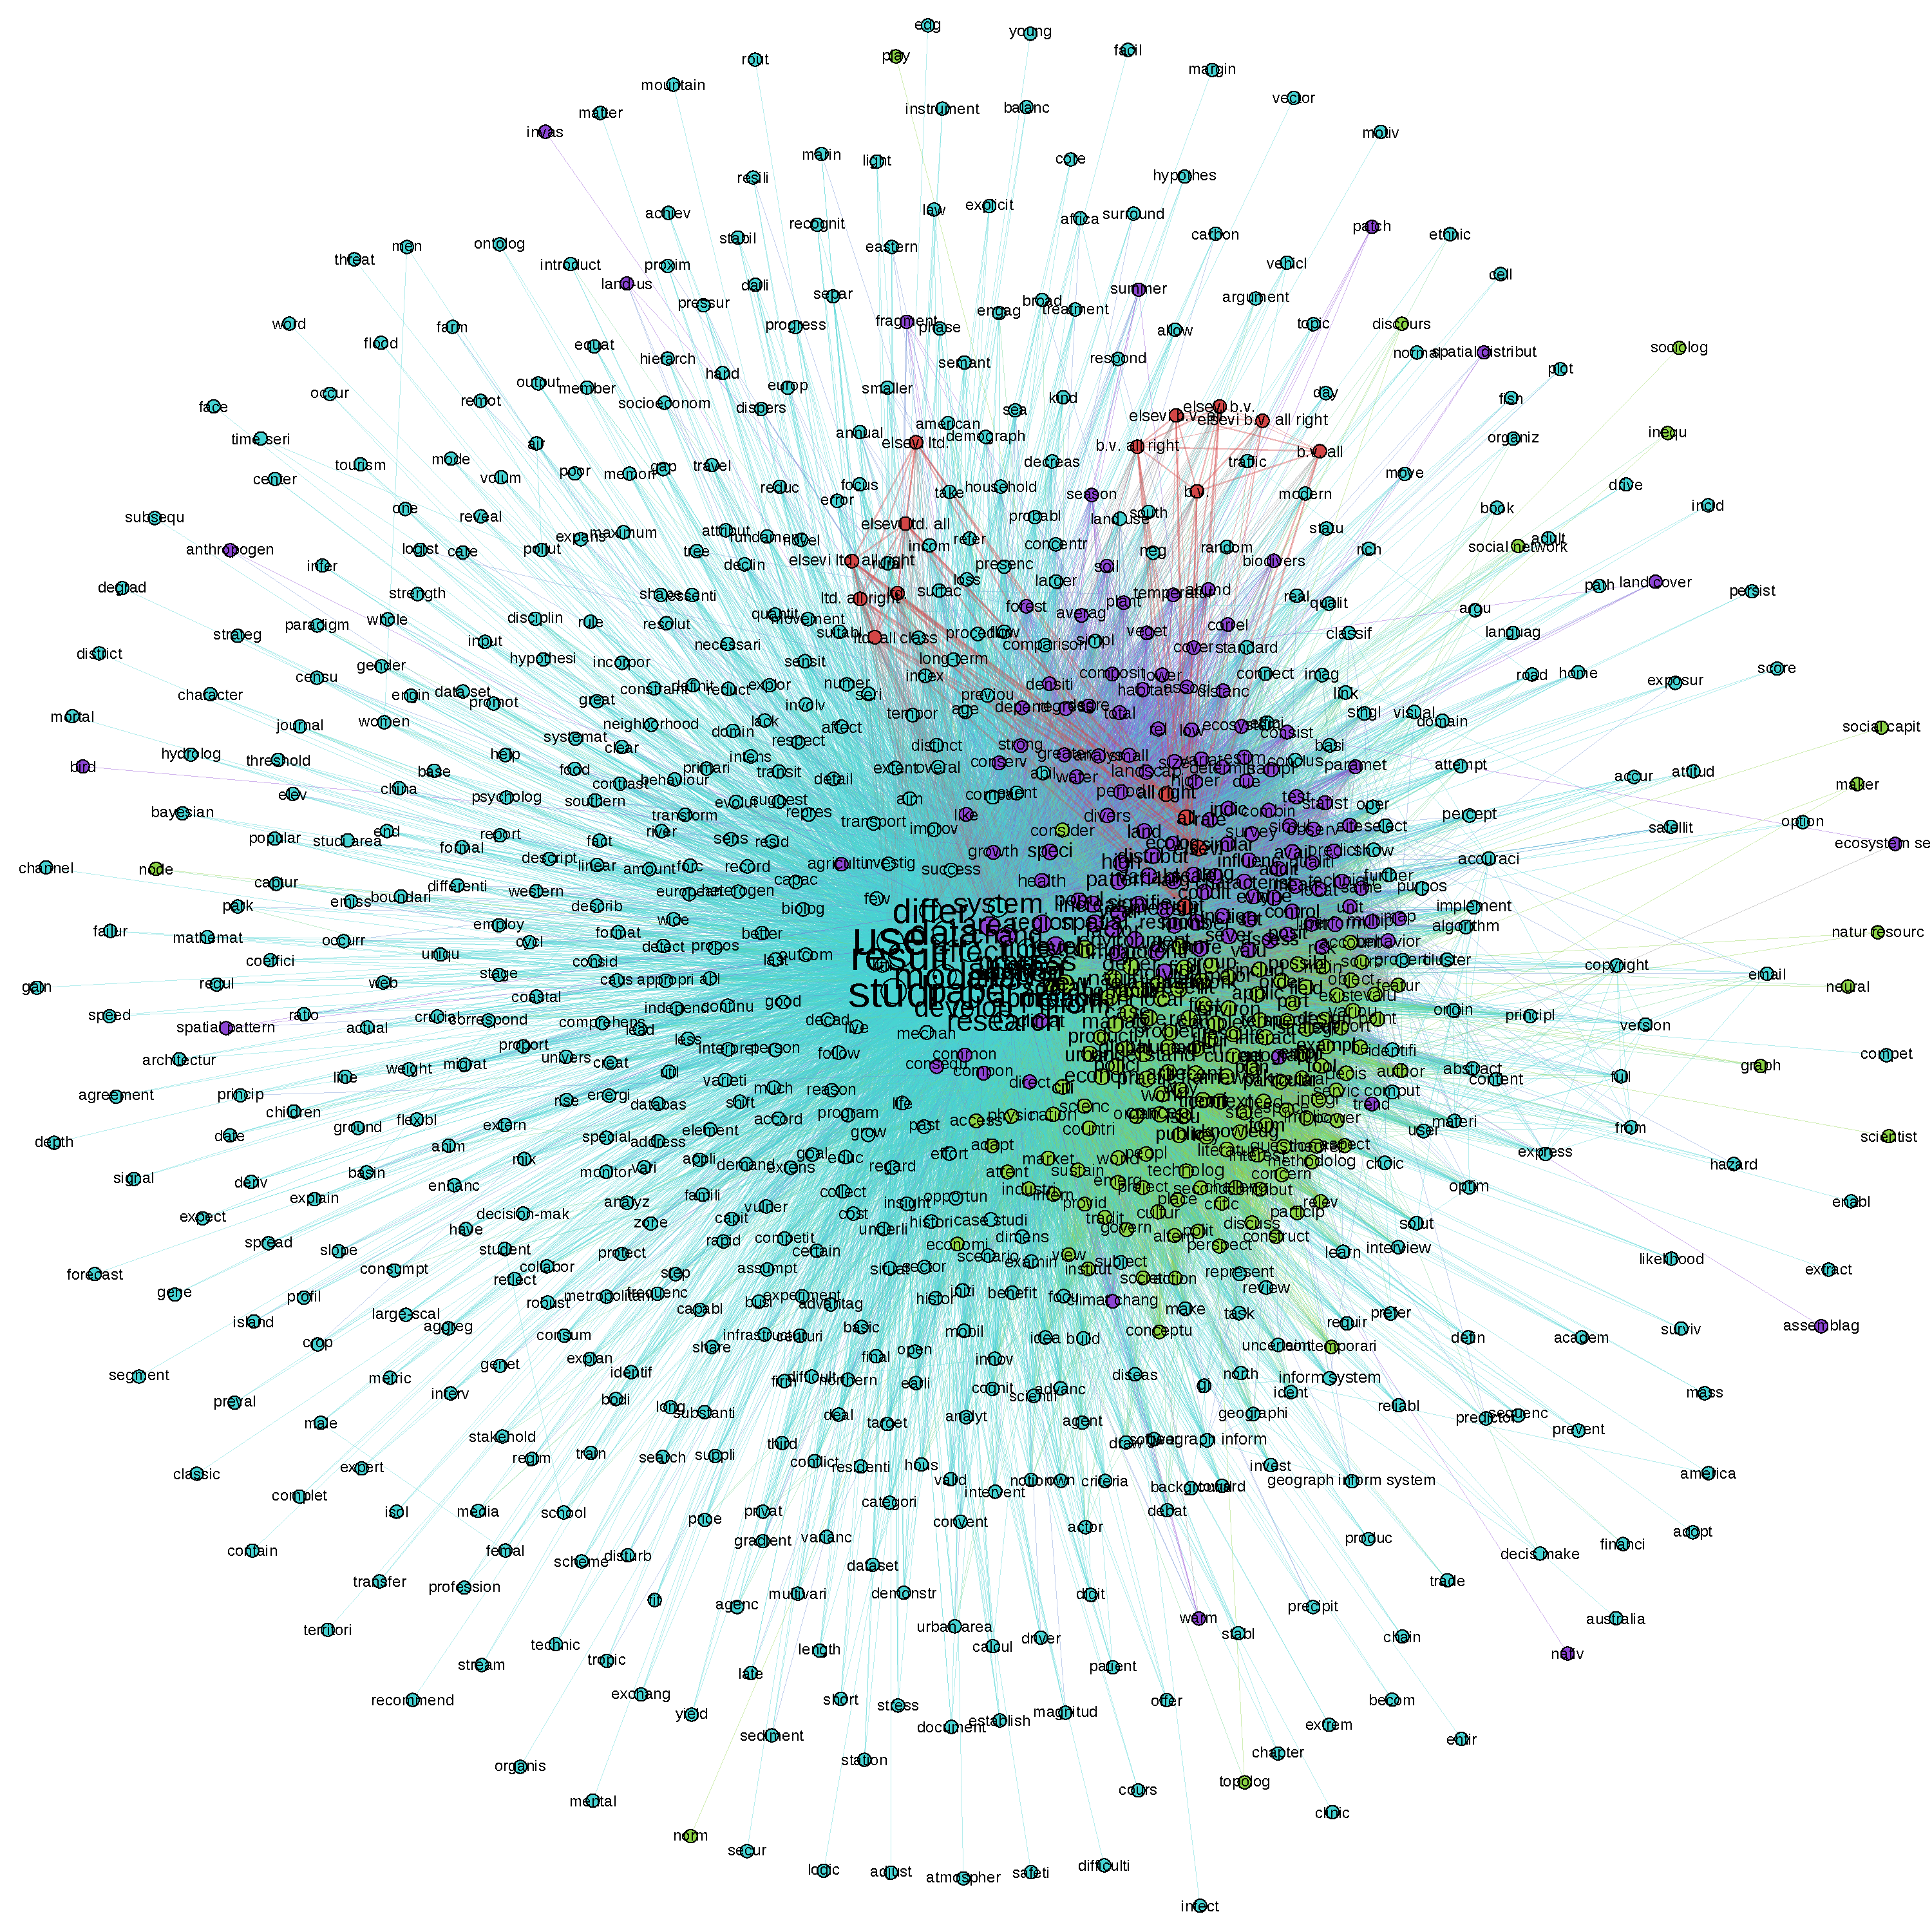
\includegraphics[height=\textheight]{figures/filt_kmin0_kmax1200_edge200}
%}
%
%
%
%\jframe{R{\'e}seau s{\'e}mantique : corpus complet (avec filtrage)}{
%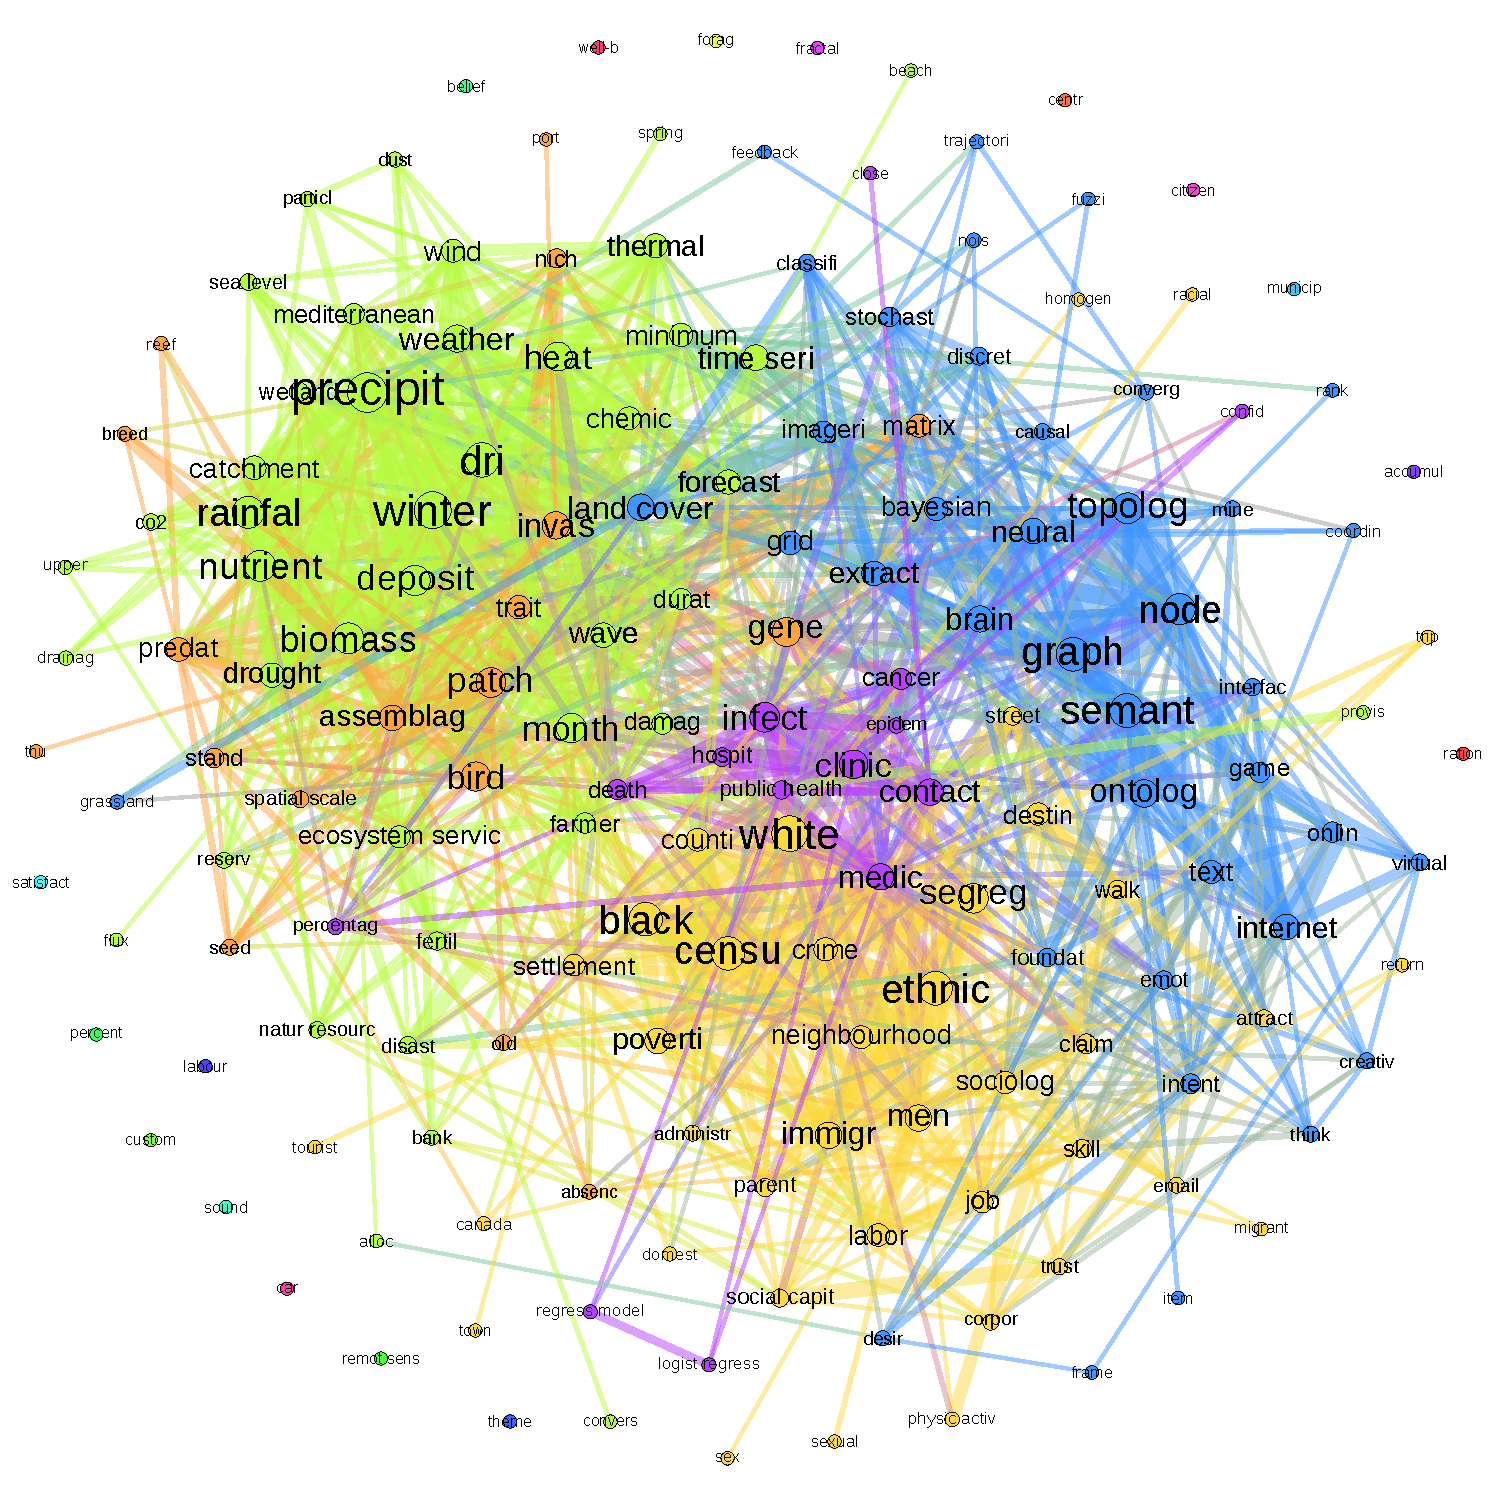
\includegraphics[height=\textheight]{figures/semanticAll}
%}
%
%
%\jframe{R{\'e}seau s{\'e}mantique : corpus cybergeo}{
%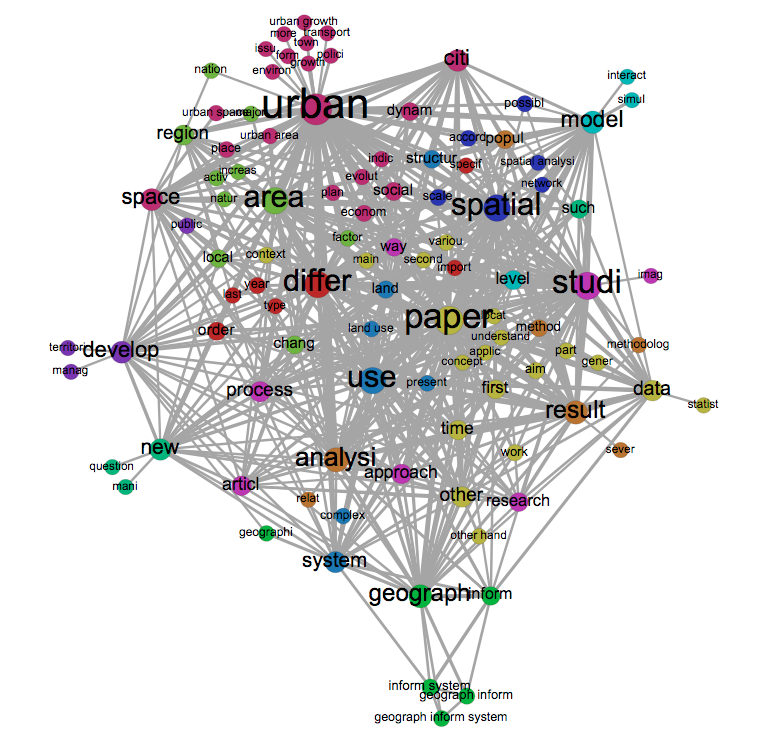
\includegraphics[height=\textheight]{figures/semanticCybergeo}
%}


%\jframe{Retour au corpus complet}{
%%\textit{Importance du r{\`e}glage fin des param{\`e}tres}
%
%\centering
%%\vspace{-2cm}
%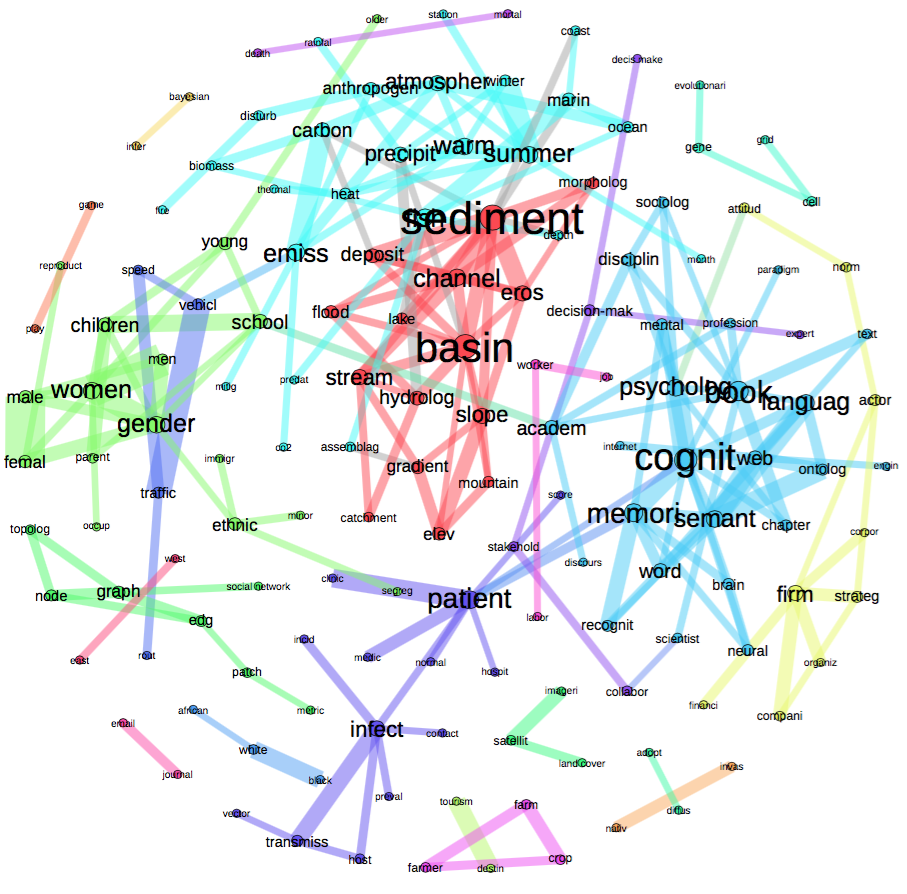
\includegraphics[height=0.9\textheight]{figures/all_lesslinks}
%}

\jframe{Influence des param{\`e}tres}{
\textit{Importance d'un r{\`e}glage fin : }

$\rightarrow$ Sensibilit{\'e} des mod{\`e}les \textbf{et} traitements de donn{\'e}es aux parametres. Exploration syst{\'e}matique via OpenMole par exemple.

$\rightarrow$ Importance du jugement d'expert : pas de dichotomie ``quanti-quali''

%$\rightarrow$ Sensibilit{\'e} aux conditions initiales : \textit{Space matters}~\cite{cottineau2015revisiting}

\medskip

\centering

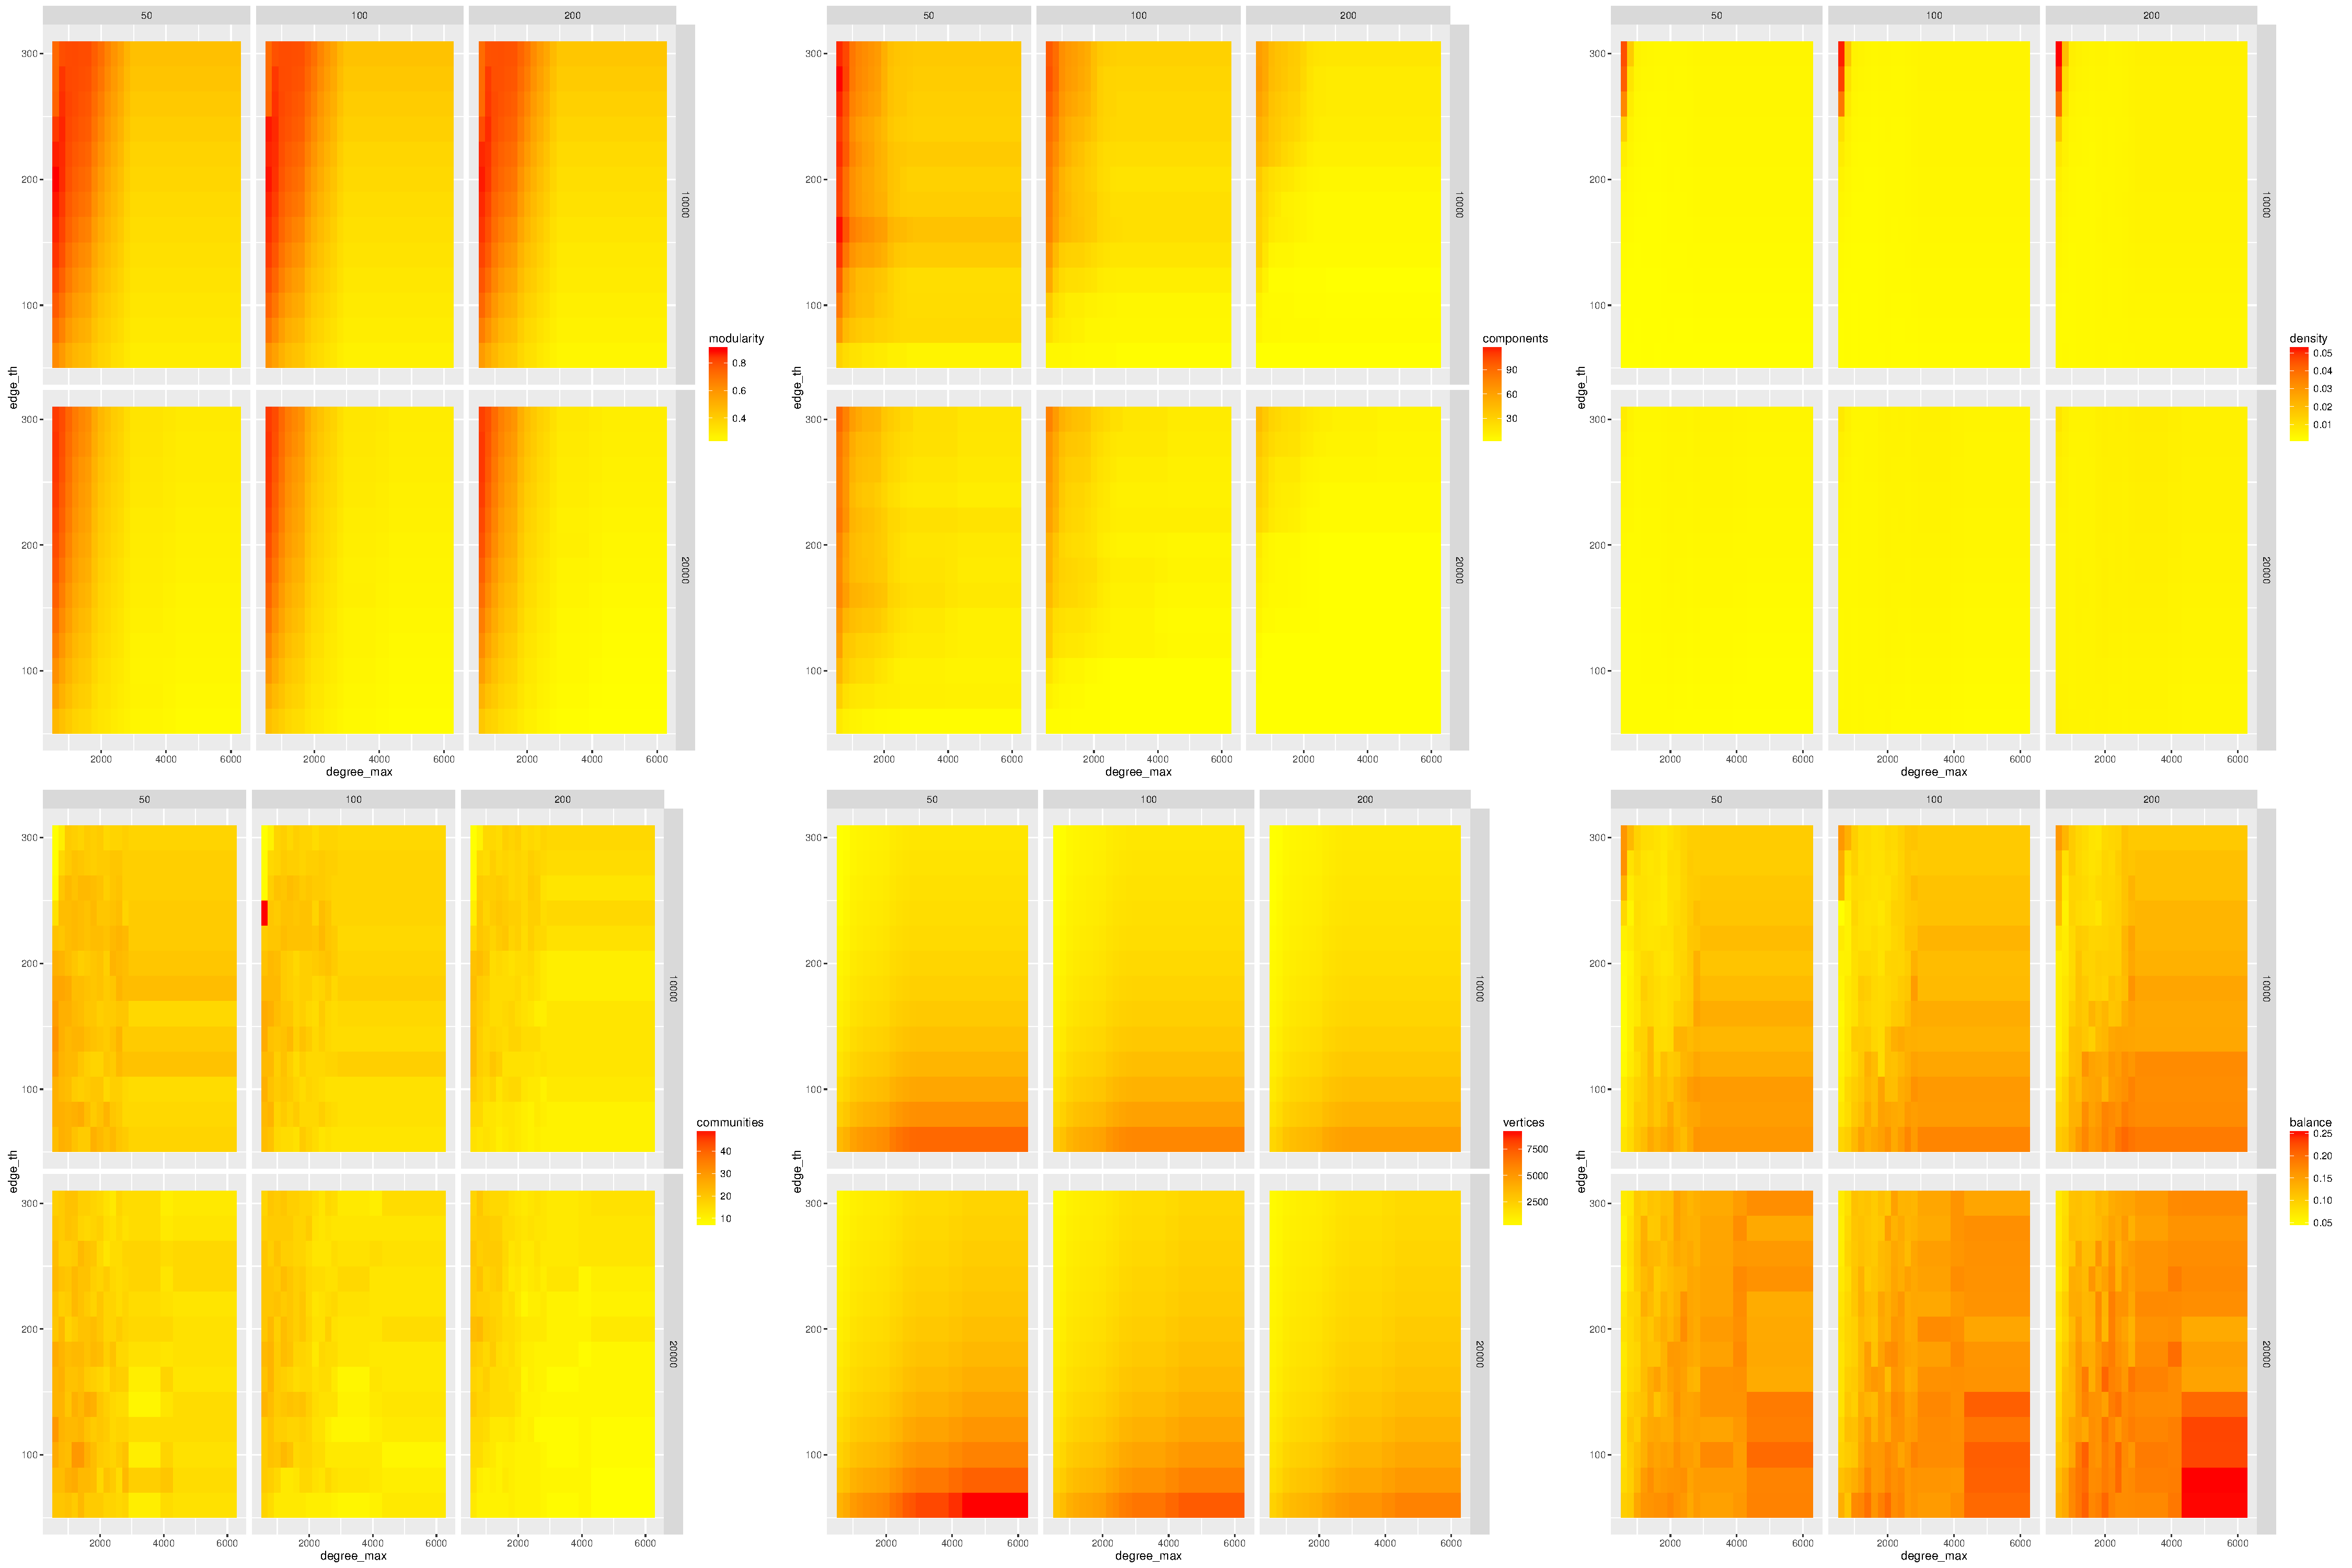
\includegraphics[width=0.65\textwidth]{figures/sensitivity_facet_allindics}


}

%\jframe{Application}{
%%\textit{Importance du r{\`e}glage fin des param{\`e}tres}
%
%\centering
%%\vspace{-2cm}
%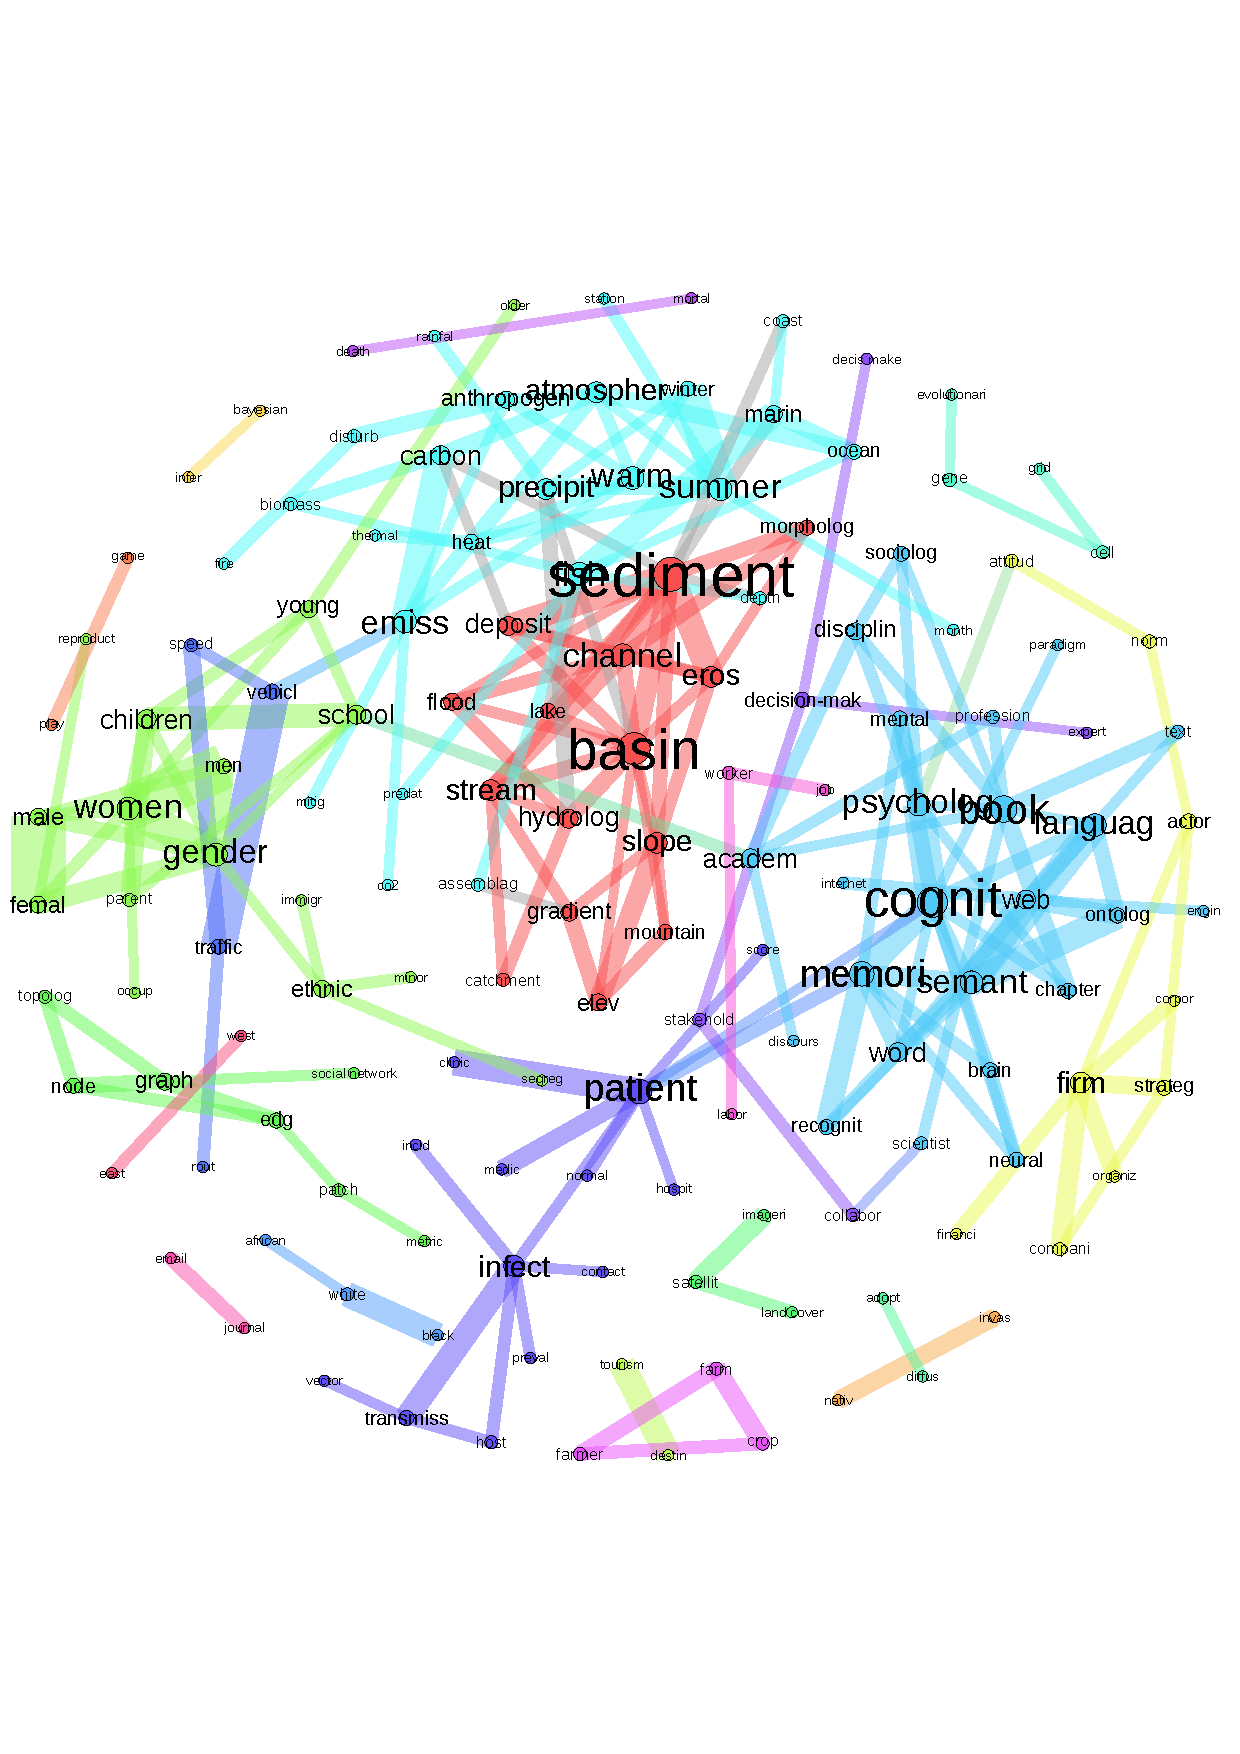
\includegraphics[height=0.9\textheight]{figures/filt_kmin5_kmax900_edge50}
%}


\jframe{Domaines extraits}{
\textit{Communaut{\'e}s obtenues pour $\theta_V=1200,\theta_E=50$ :}
\bigskip
{\footnotesize
\begin{itemize}
\item Political sciences/critical geography (535) : \texttt{decision-mak, polit ideolog, democraci, stakehold, neoliber}
\item Biogeography (394) : \texttt{plant densiti, wood, wetland, riparian veget}
\item Economic geography (343) : \texttt{popul growth, transact cost, socio-econom, household incom}
\item Environnment/climate (309) : \texttt{ice sheet, stratospher, air pollut, climat model}
\item Complex systems (283) : \texttt{scale-fre, multifract, agent-bas model, self-organ}
\item Physical geography (203) : \texttt{sedimentari, digit elev model, geolog, river delta}
\item Spatial analysis (175) : \texttt{spatial analysi, princip compon analysi, heteroscedast, factor analysi}
\end{itemize}
}
}

\jframe{Domaines extraits (suite)}{
{\footnotesize
\begin{itemize}
\item Microbiology (118) : \texttt{chromosom, phylogenet, borrelia}
\item Statistical methods (88) : \texttt{logist regress, classifi, kalman filter, sampl size}
\item Cognitive sciences (81) : \texttt{semant memori, retrospect, neuroimag}
\item GIS (75) : \texttt{geograph inform scienc, softwar design, volunt geograph inform, spatial decis support}
\item Traffic modeling (63) : \texttt{simul model, lane chang, traffic flow, crowd behavior}
\item Health (52) : \texttt{epidem, vaccin strategi, acut respiratori syndrom, hospit}
\item Remote sensing (48) : \texttt{land-cov, landsat imag, lulc}
\item Crime (17) : \texttt{crimin justic system, social disorgan, crime}
\end{itemize}

}
}


\jframe{R{\'e}seau}{
\centering
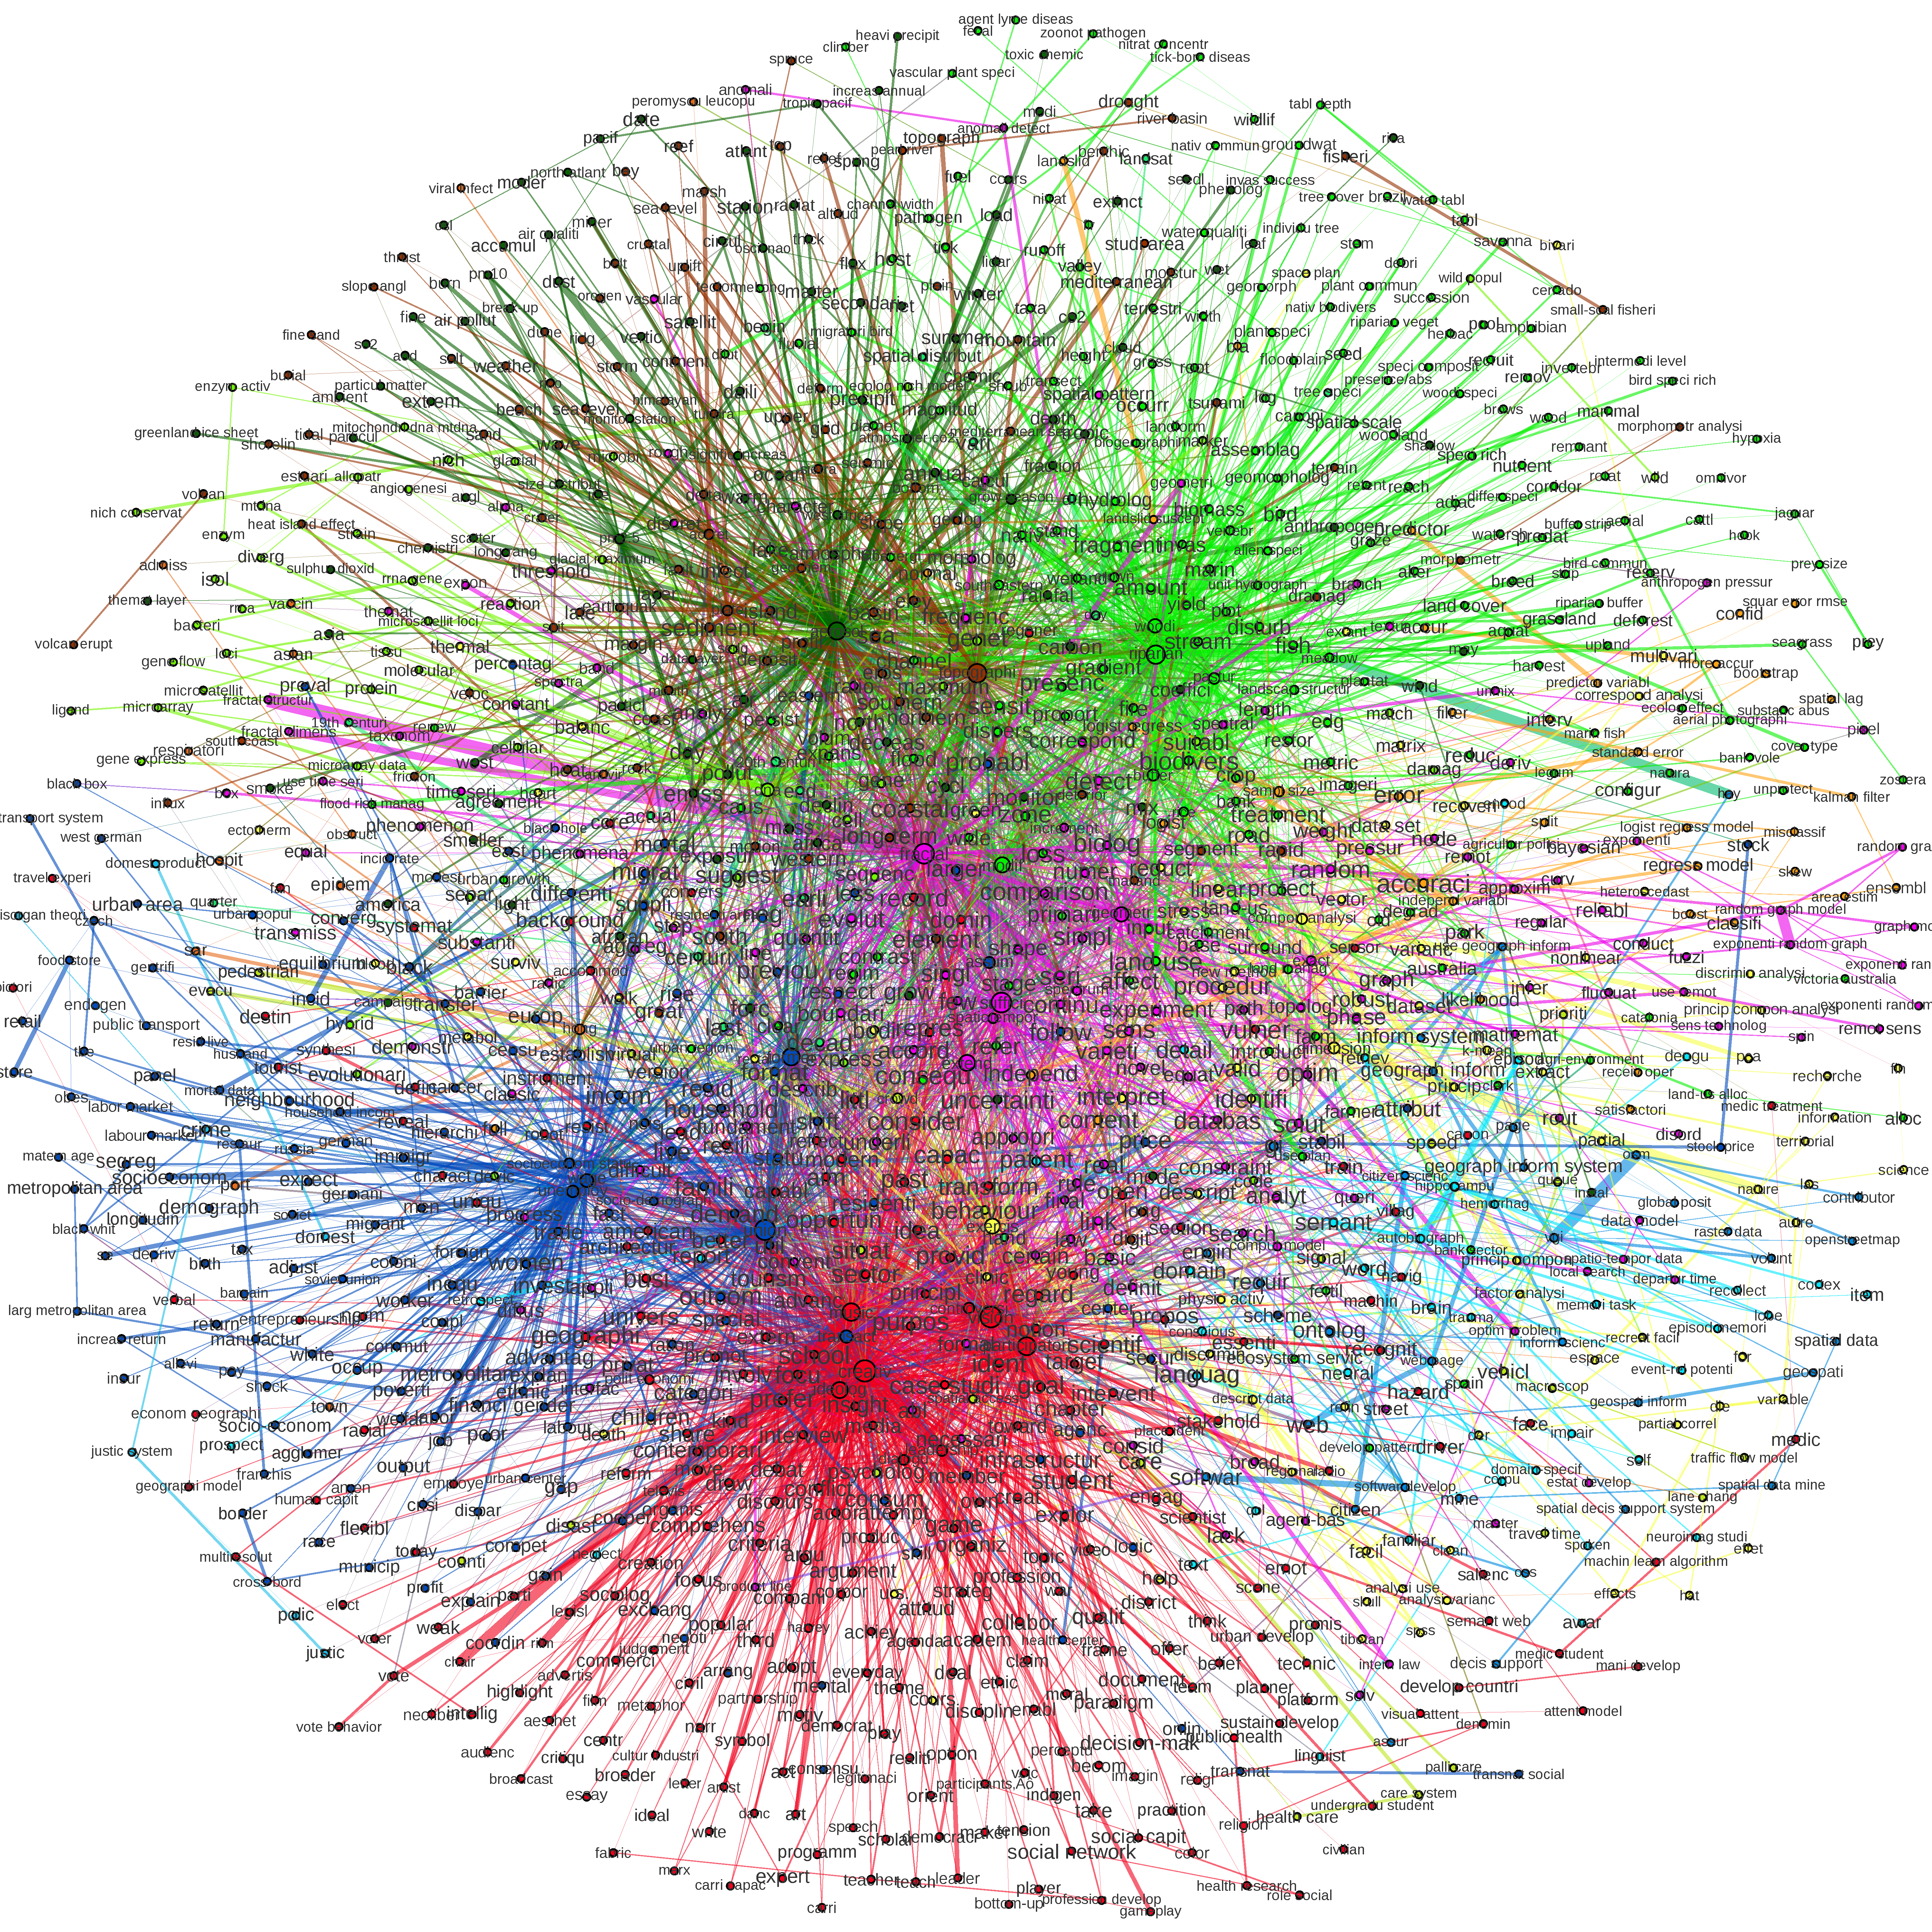
\includegraphics[height=0.85\textheight]{figures/semantic.png}
}

\jframe{Interdisicplinarit{\'e}}{
\centering
\includegraphics[height=0.85\textheight]{figures/synththemcyb}
}


\jframe{Interdisicplinarit{\'e} de citation}{
\centering
%\vspace{-1.5cm}
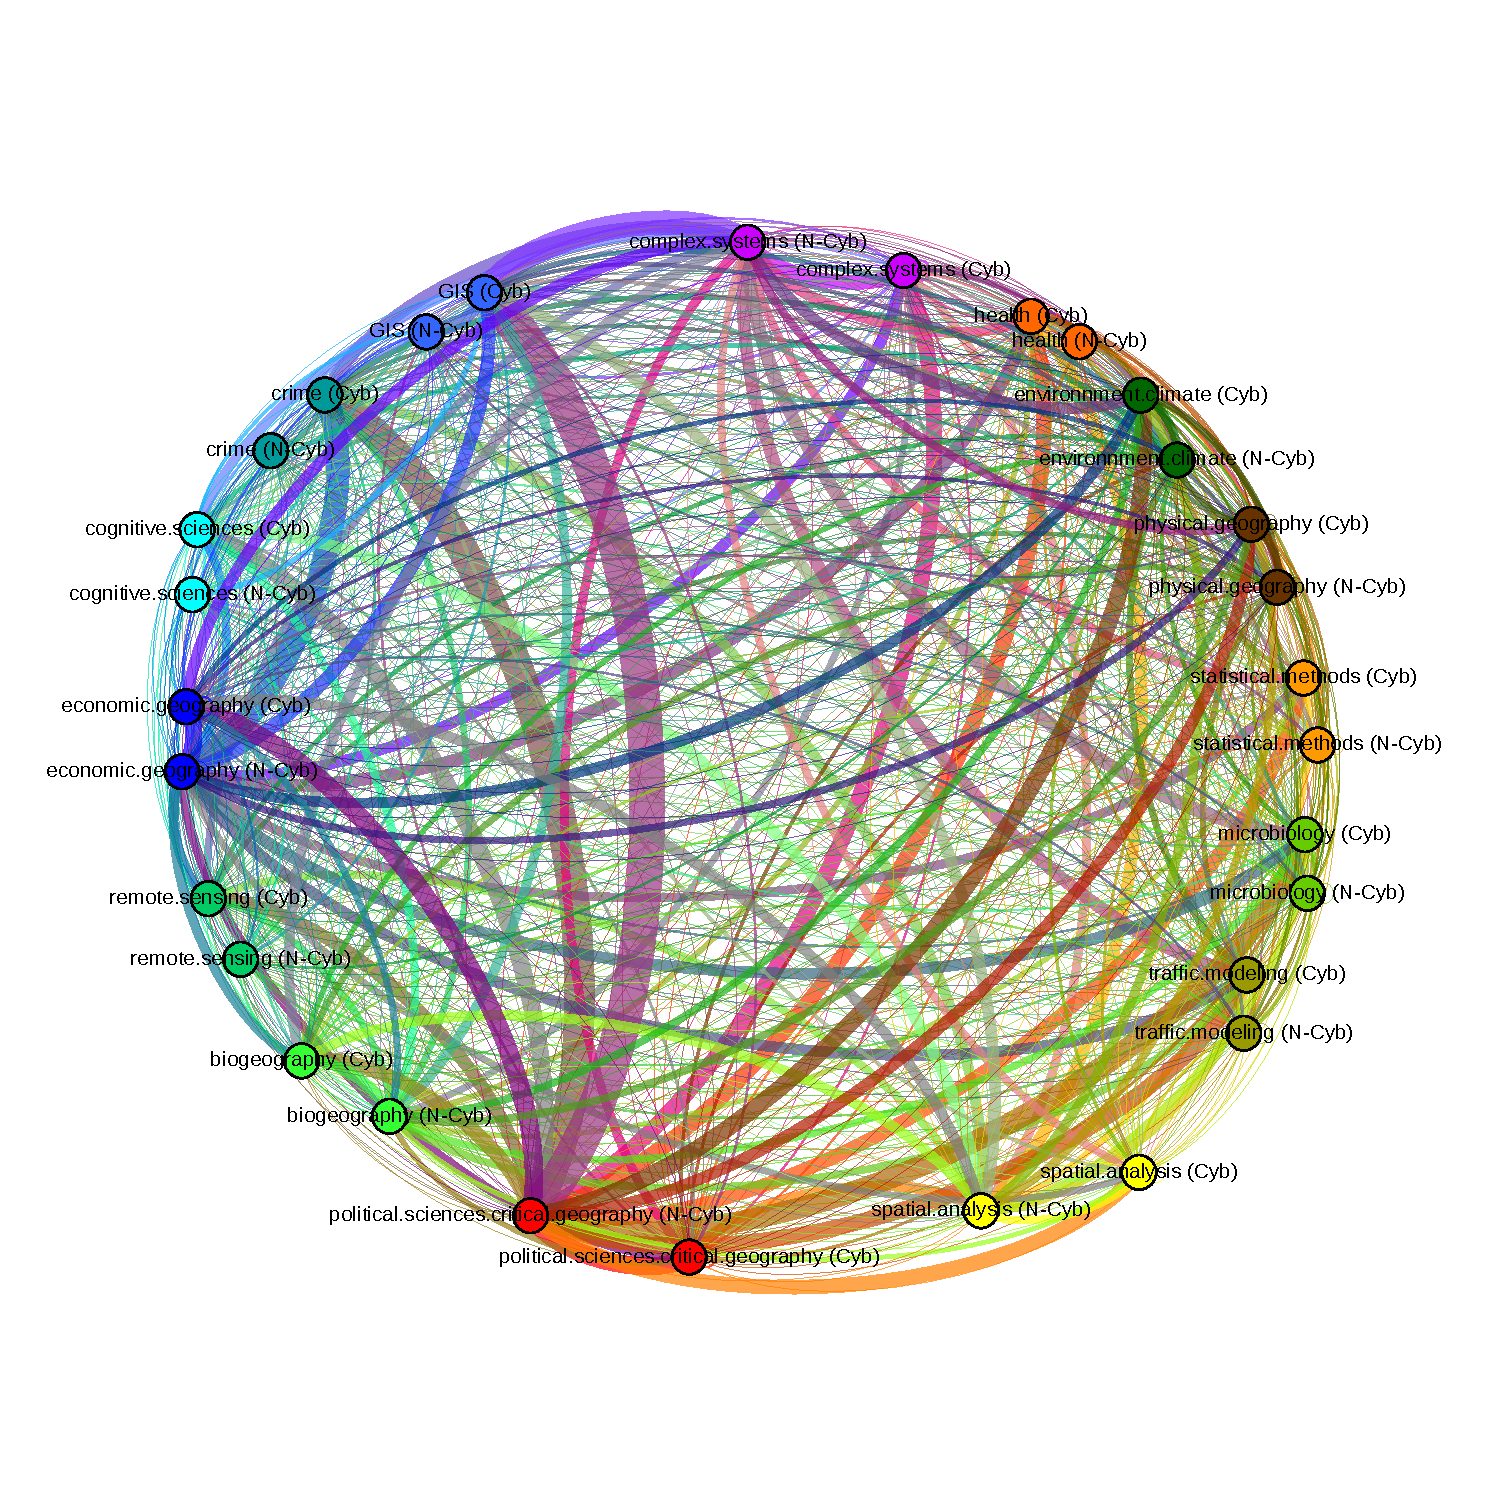
\includegraphics[height=0.9\textheight]{figures/citation}
}




\jframe{Degr{\'e} d'interdisciplinarit{\'e} par articles}{
Un article peut {\^e}tre associ{\'e} aux communaut{\'e}s s{\'e}mantiques par ses mots cl{\'e}s : probas $p_i$ pour chaque communaut{\'e}.

Mesure d'interdisciplinarit{\'e} (pour un article, au premier ordre) :
\[
o = 1 - \sum p_i^2
\]

\centering

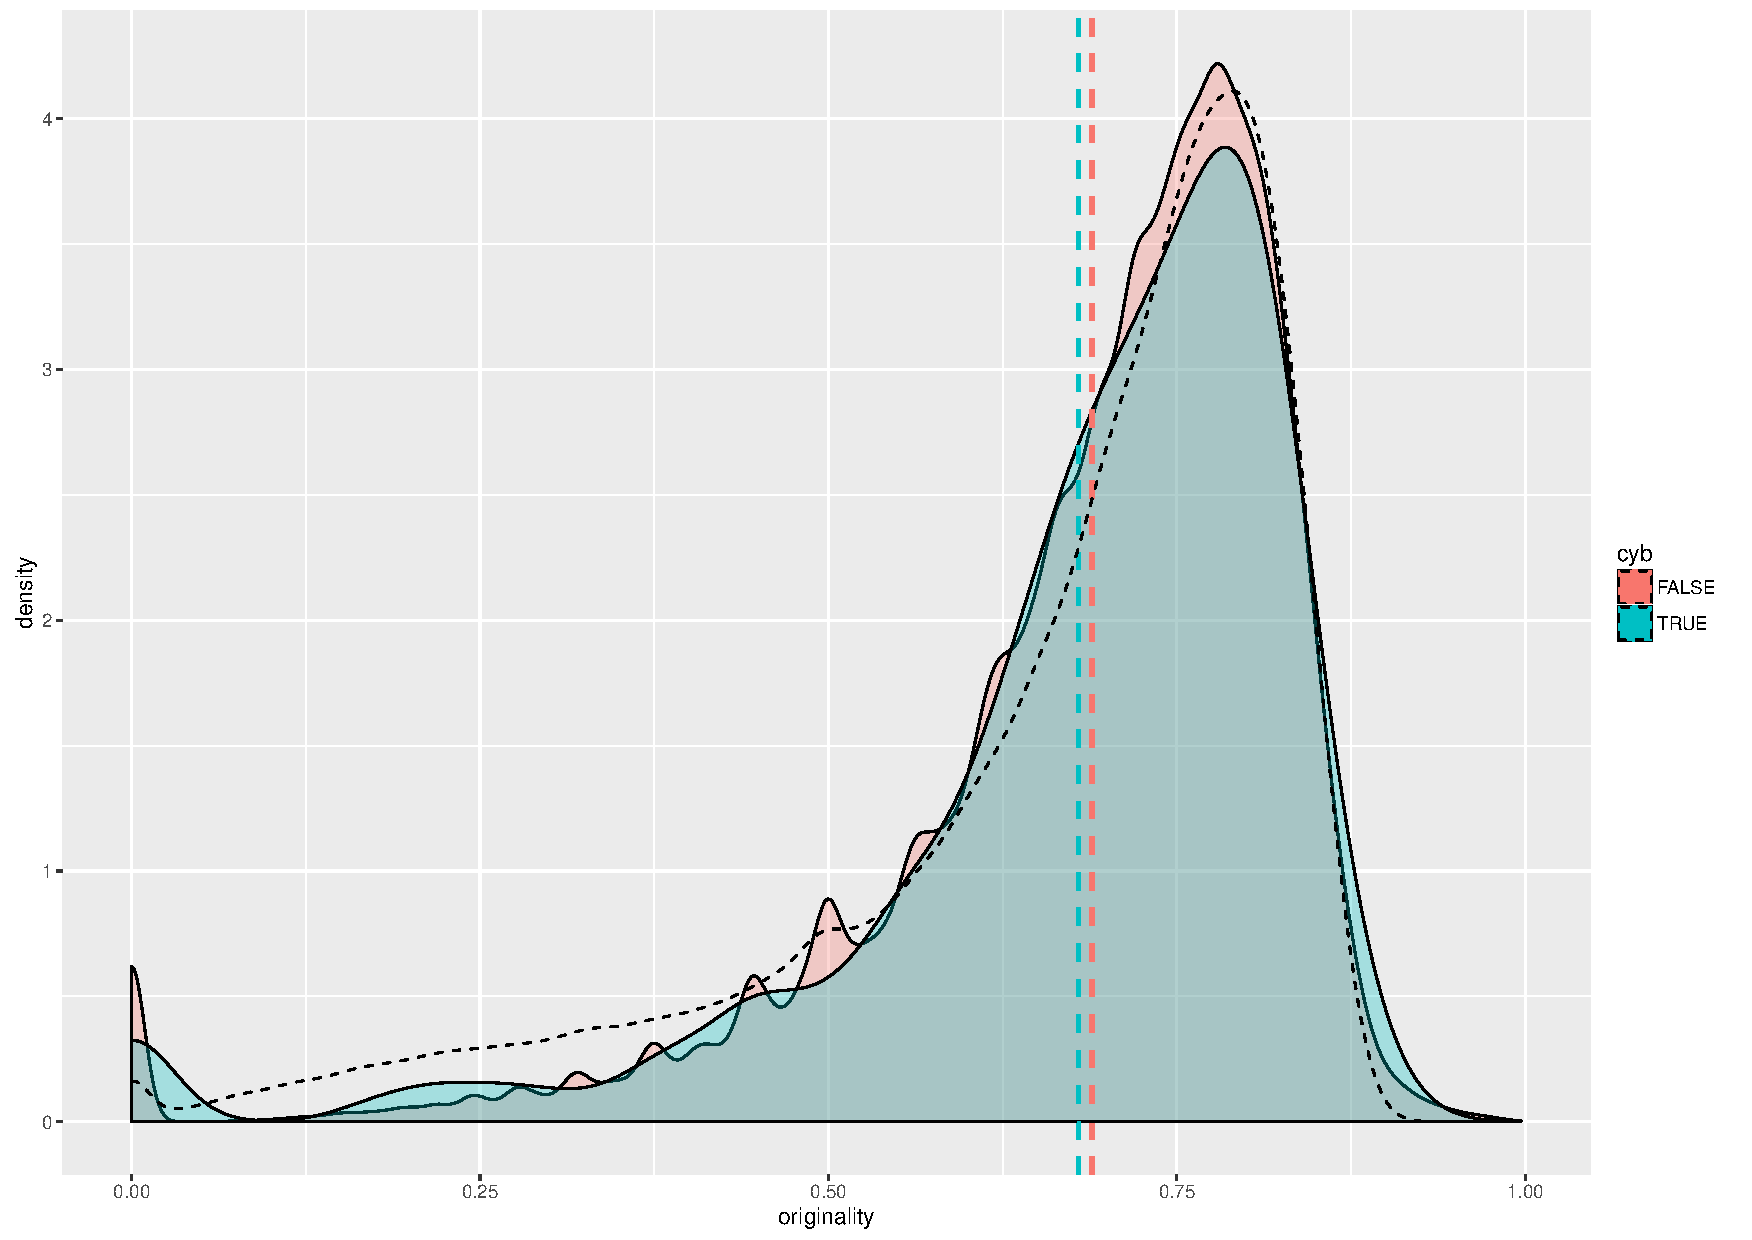
\includegraphics[width=0.5\textwidth]{figures/firstorderint_withNull}

}

\jframe{Interdisciplinarit{\'e} de citation}{

\centering

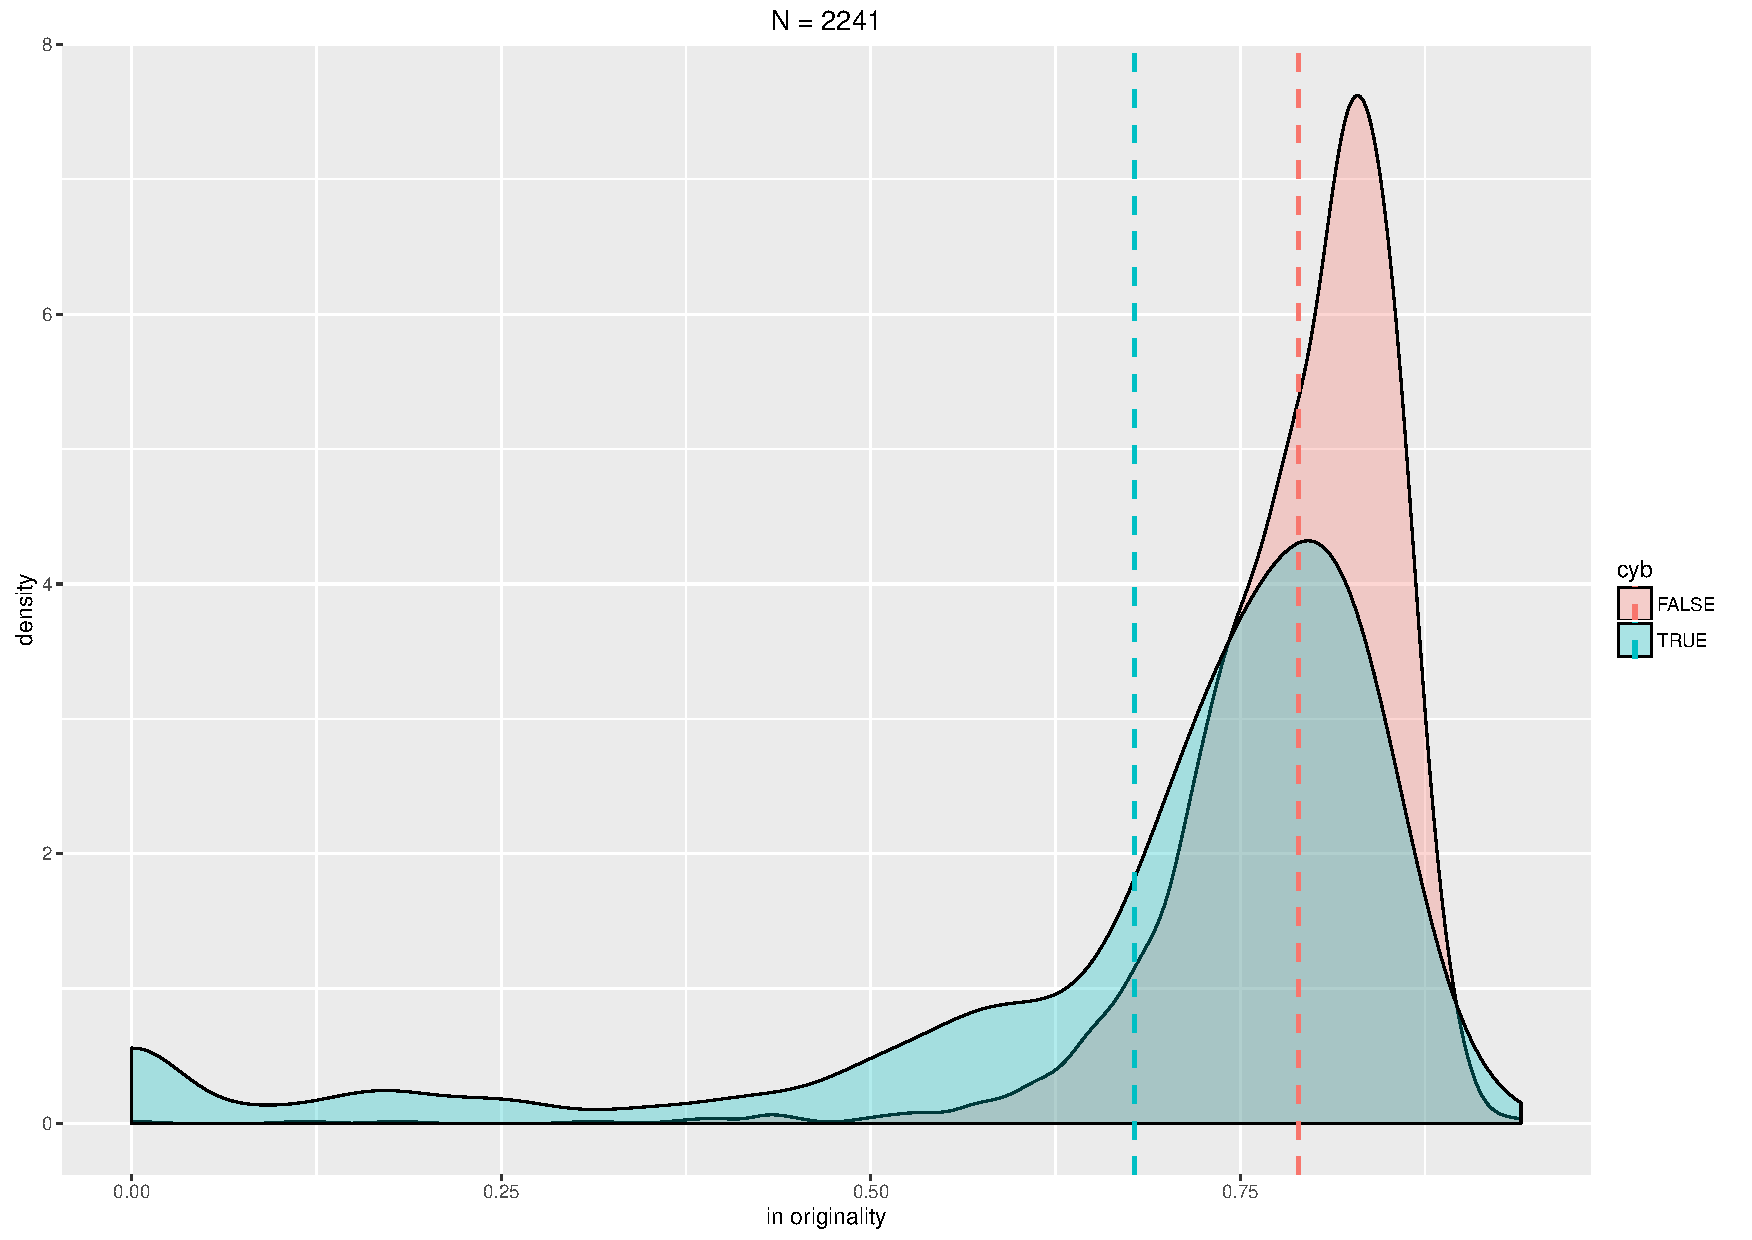
\includegraphics[width=0.45\textwidth]{figures/citin_interdisc}
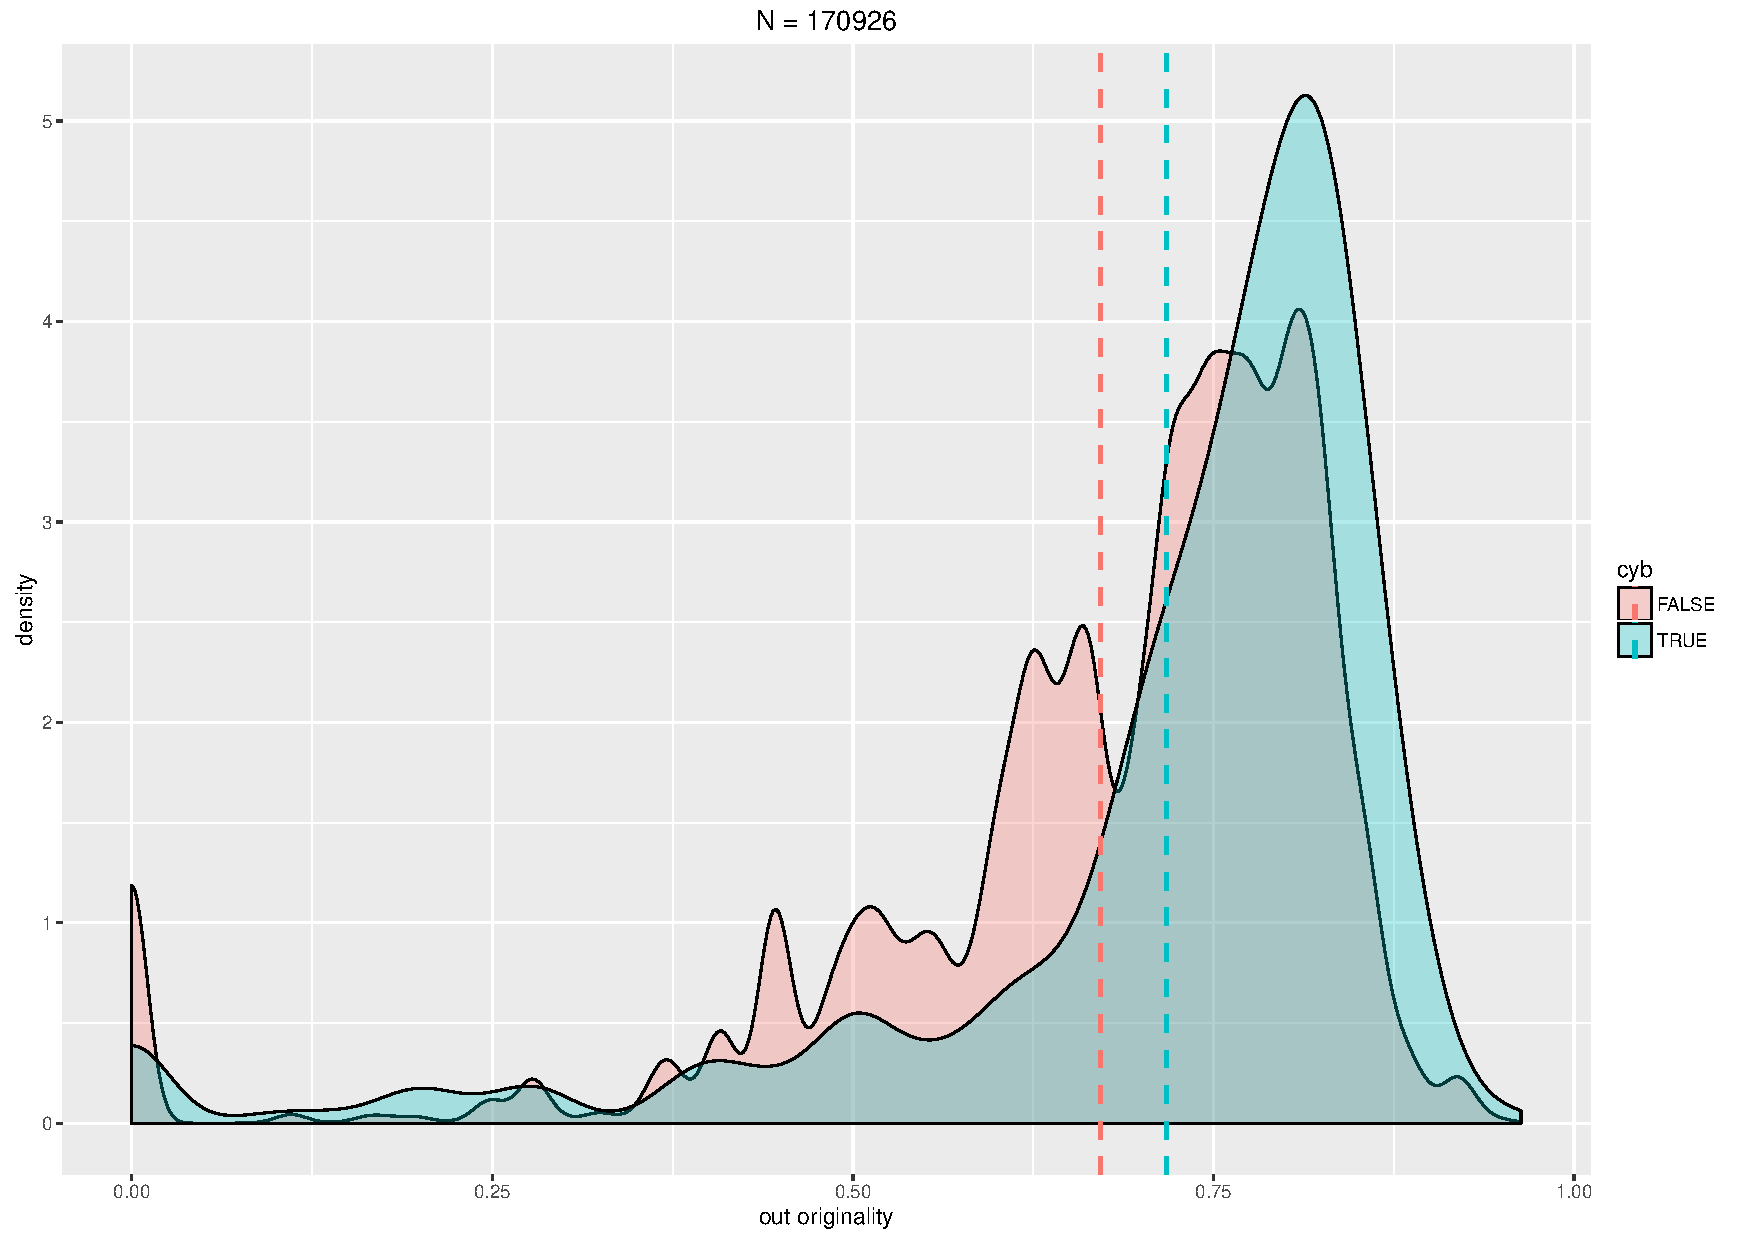
\includegraphics[width=0.45\textwidth]{figures/citout_interdisc}


}

%\jframe{Degr{\'e} d'interdisciplinarit{\'e}}{
%
%Aggregation au niveau de la revue : originalit{\'e} des th{\`e}mes abord{\'e}s dans l'ensemble de la revue
%
%\[
%O = 1 - \sum_i \left[\frac{1}{K}\sum_k p_i^{(k)}\right]^2
%\]
%
%$\rightarrow$ 0.890 pour cybergeo (0.8933 pour un mod{\`e}le nul par tirage al{\'e}atoire)
%
%\textit{Besoin d'autres revues pour comparaison : retour {\`a} la collecte de donn{\'e}es}
%
%
%}
%
%\jframe{Interdisciplinarit{\'e} au second ordre}{
%
%\textit{Croisement des couches de l'hyperr{\'e}seau.}
%
%$\rightarrow$ Originalit{\'e} de l'ensemble des voisins (entrants ou sortants) dans le r{\'e}seau de citation
%
%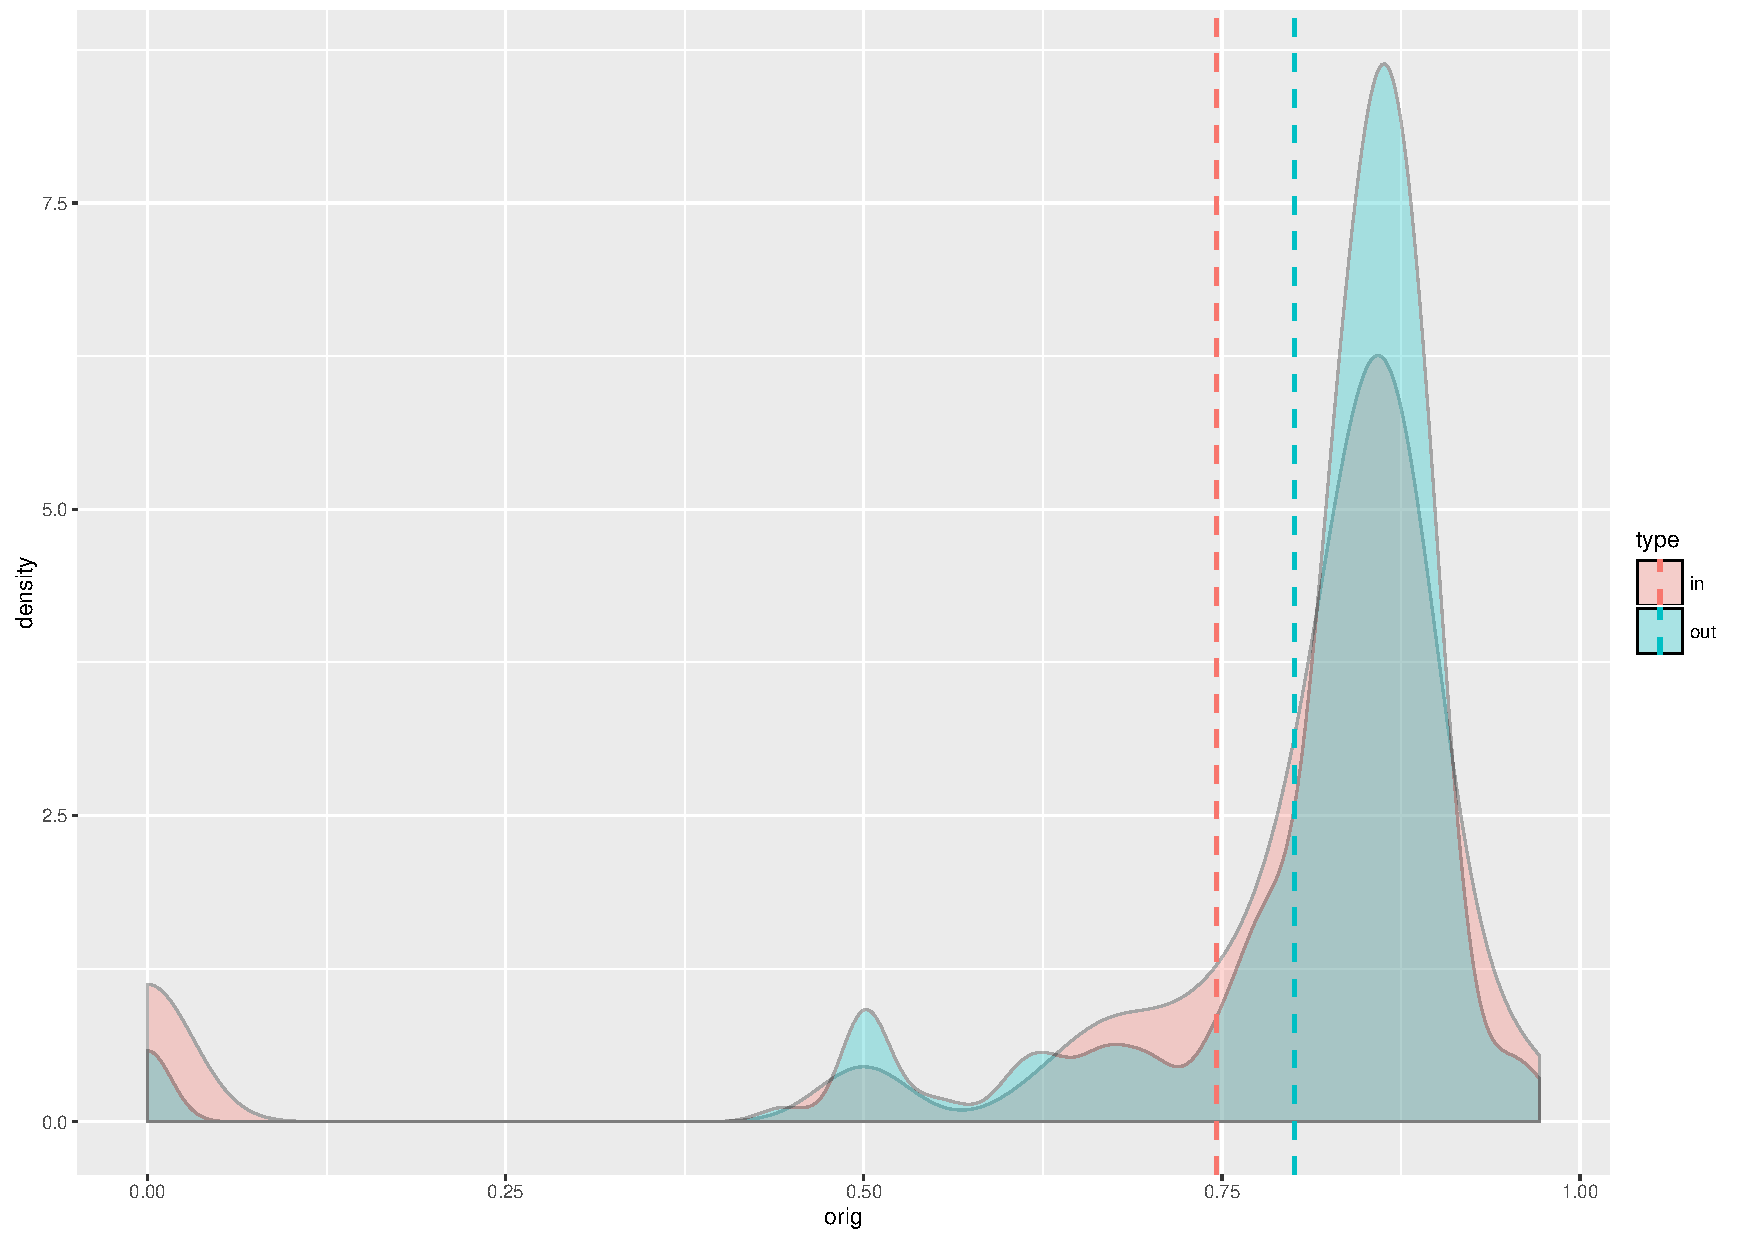
\includegraphics[width=0.7\textwidth]{figures/2ndorderOrig}
%
%
%}



\jframe{Conclusion}{
  $\rightarrow$ Un environnement disciplinaire tr{\`e}s vari{\'e} et une interdicisplinarit{\'e} affirm{\'e}e
  
  \bigskip
  
  $\rightarrow$ Approche {\`a} croiser avec autres types de classifications (th{\'e}matique (POC), mots-cl{\'e}s (HC), g{\'e}ographique (CC) pour en apprendre plus sur la revue et la pratique de la g{\'e}ographie qui lui est associ{\'e}e
  \bigskip
  
  $\rightarrow$ M{\'e}thode g{\'e}n{\'e}rique pouvant s'appliquer {\`a} tout r{\'e}seau dont les noeuds ont une description textuelle
}



%
%\jframe{Perspectives}{
%Attention {\`a} la tentation des \textit{big data} et de la simulation {\`a} outrance : garder un ancrage th{\'e}orique (poser les bonnes questions) et m{\'e}thodologique.
%
%\bigskip
%
%Exemple : travail en cours sur interactions Ville/Transports : donn{\'e}es ``simples'' et classiques (densit{\'e} population et OSM), statiques, fournissent de l'information sur processus dynamiques sous-jacents. N{\'e}cessit{\'e} du cadre th{\'e}orique (th{\'e}orie {\'e}volutive des villes) et du travail m{\'e}thodologique pour relier statique-dynamique.
%}
%
%\jframe{Conclusion ({\`a} retenir)}{
%\begin{itemize}
%\item ``Big Data'' plus que relatif
%\bigskip
%\item Des donn{\'e}es partout, {\`a} vous de les collecter et cr{\'e}er des bases \textbf{ouvertes} (pas de science sans ouverture : multimodeling et open science)
%\bigskip
%\item G{\'e}ographie {\`a} la pointe de par les connaissances d{\'e}j{\`a} pr{\'e}sentes : {\`a} vous de jouer !
%\end{itemize}
%}
%



\jframe{Reserve Slides}{
\Large \textit{Reserve Slides}
}





\jframe{Collecte des donn{\'e}es}{
\textit{Crawling de donn{\'e}es semi-ouvertes : exemples en g{\'e}ographie}

\bigskip

Donn{\'e}es de mobilit{\'e} : statuts des stations Vlib en temps r{\'e}el (API)

\cite{raimbault2015user}

\bigskip

\centering
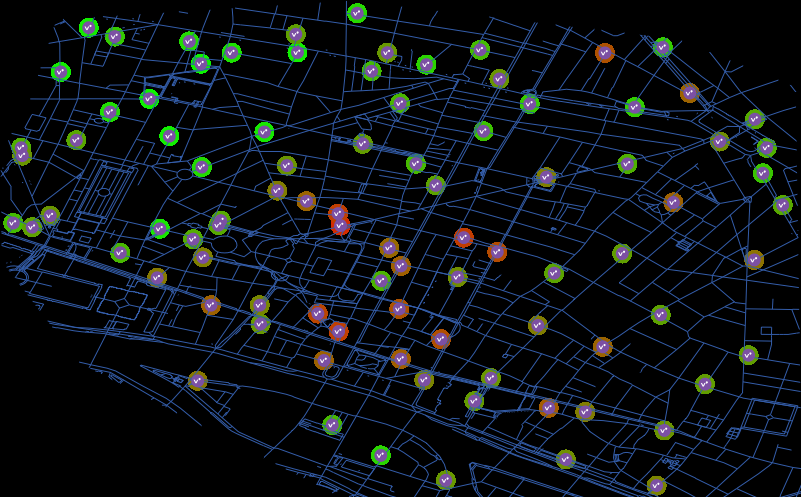
\includegraphics[width=0.7\textwidth]{figures/velib}



}

\jframe{Collecte des donn{\'e}es}{
\textit{Exemples en g{\'e}ographie (suite)}

\bigskip

Traffic routier : collecte de \textit{sytadin} (pas d'API : \textit{scrapping} n{\'e}c{\'e}ssaire)


\bigskip

\centering
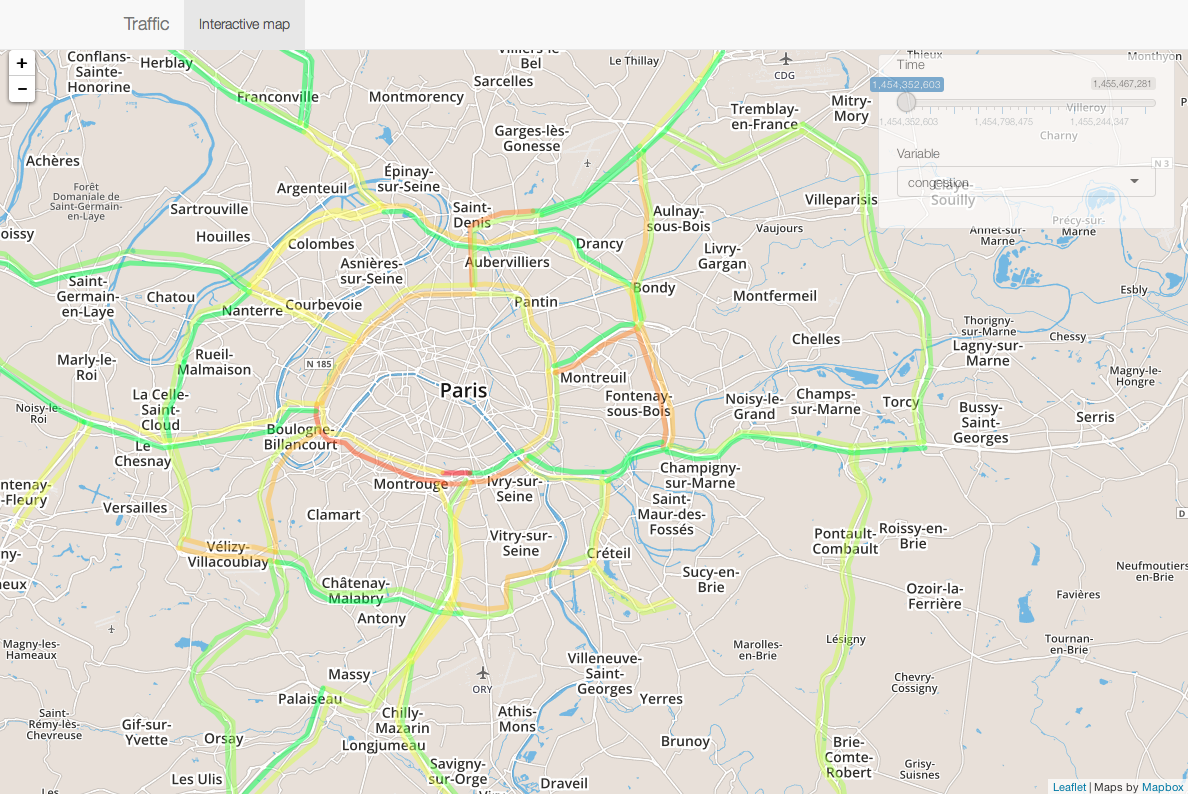
\includegraphics[width=0.8\textwidth]{figures/screen_appli}


\bigskip



}






\jframe{Centralit{\'e} (citation)}{

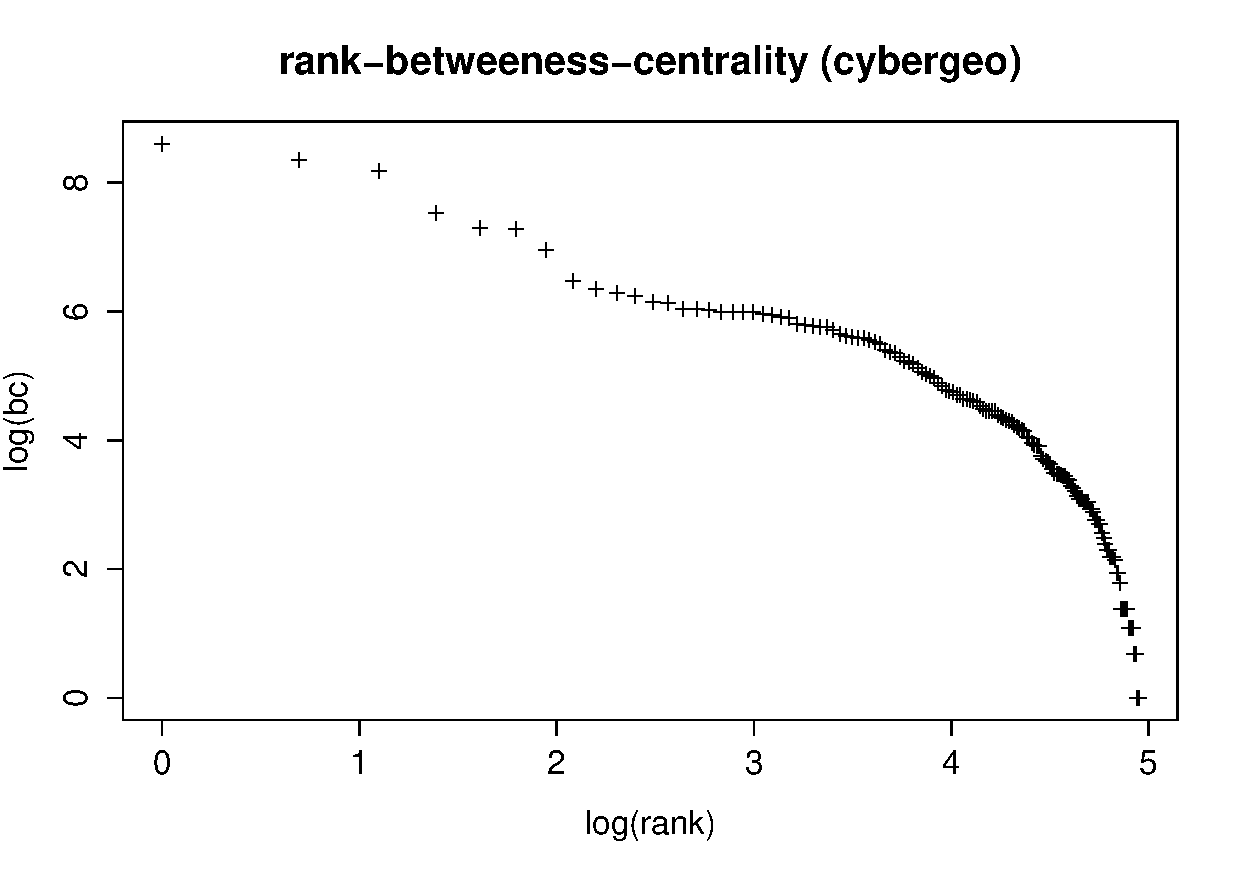
\includegraphics[width=0.5\textwidth]{figures/betweeness-cyb}
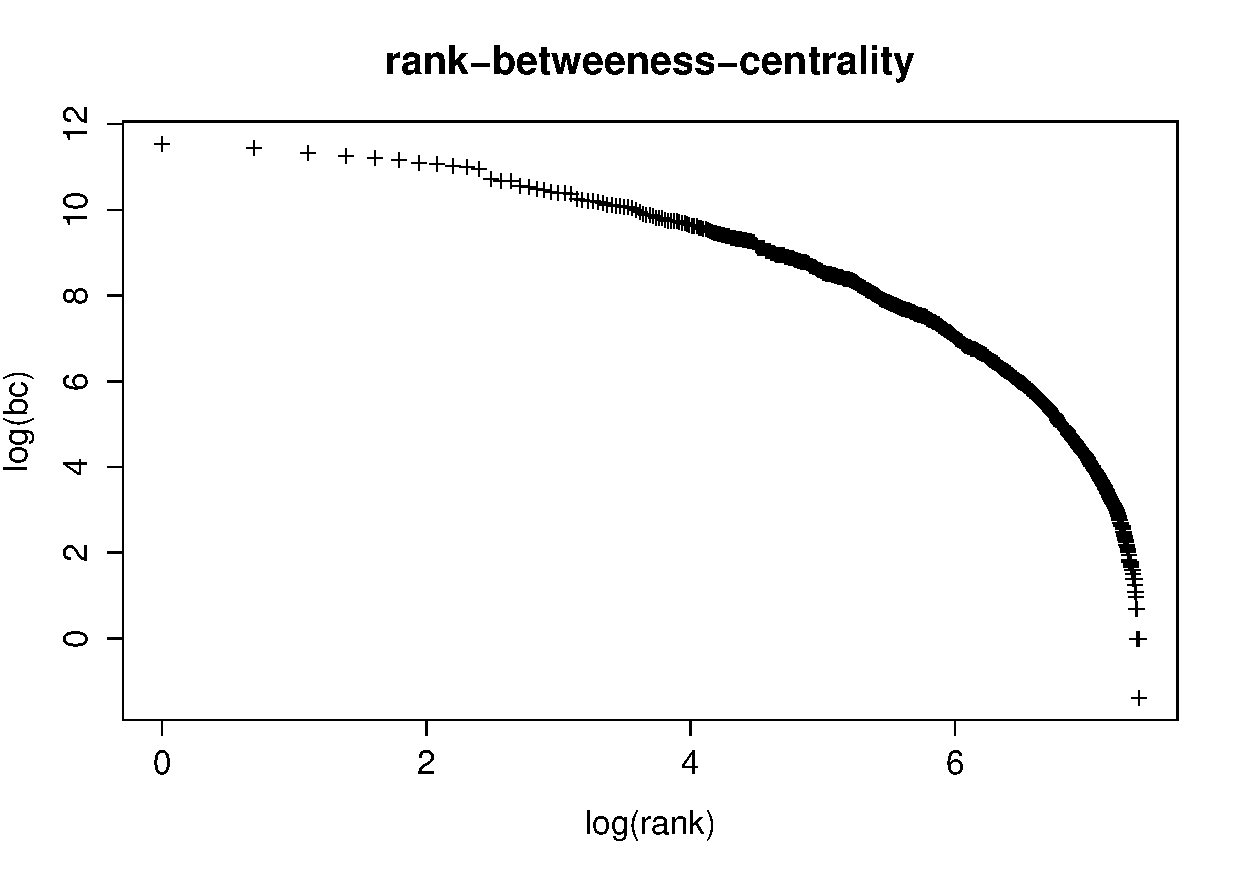
\includegraphics[width=0.5\textwidth]{figures/betweeness}

\textit{Centralit{\'e}s faibles (rq : impossibilit{\'e} des clusters forts pour des citations car causalit{\'e} temporelle). Gauche : Cyberg{\'e}o ; Droite : Ensemble du r{\'e}seau}

}


\jframe{Clustering (citation)}{
Composante g{\'e}ante : plus de 99\% des noeuds.
\medskip

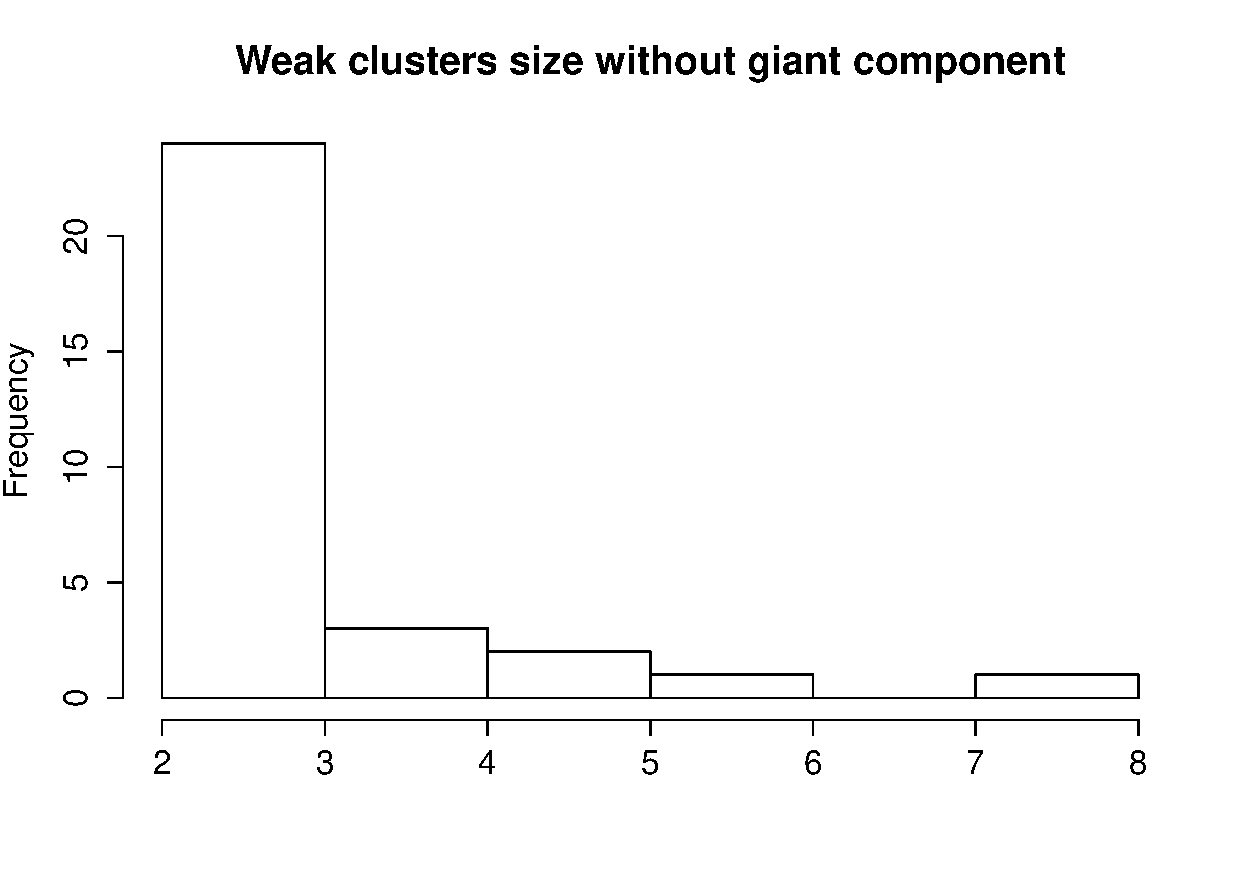
\includegraphics[width=0.5\textwidth]{figures/clusterSize}
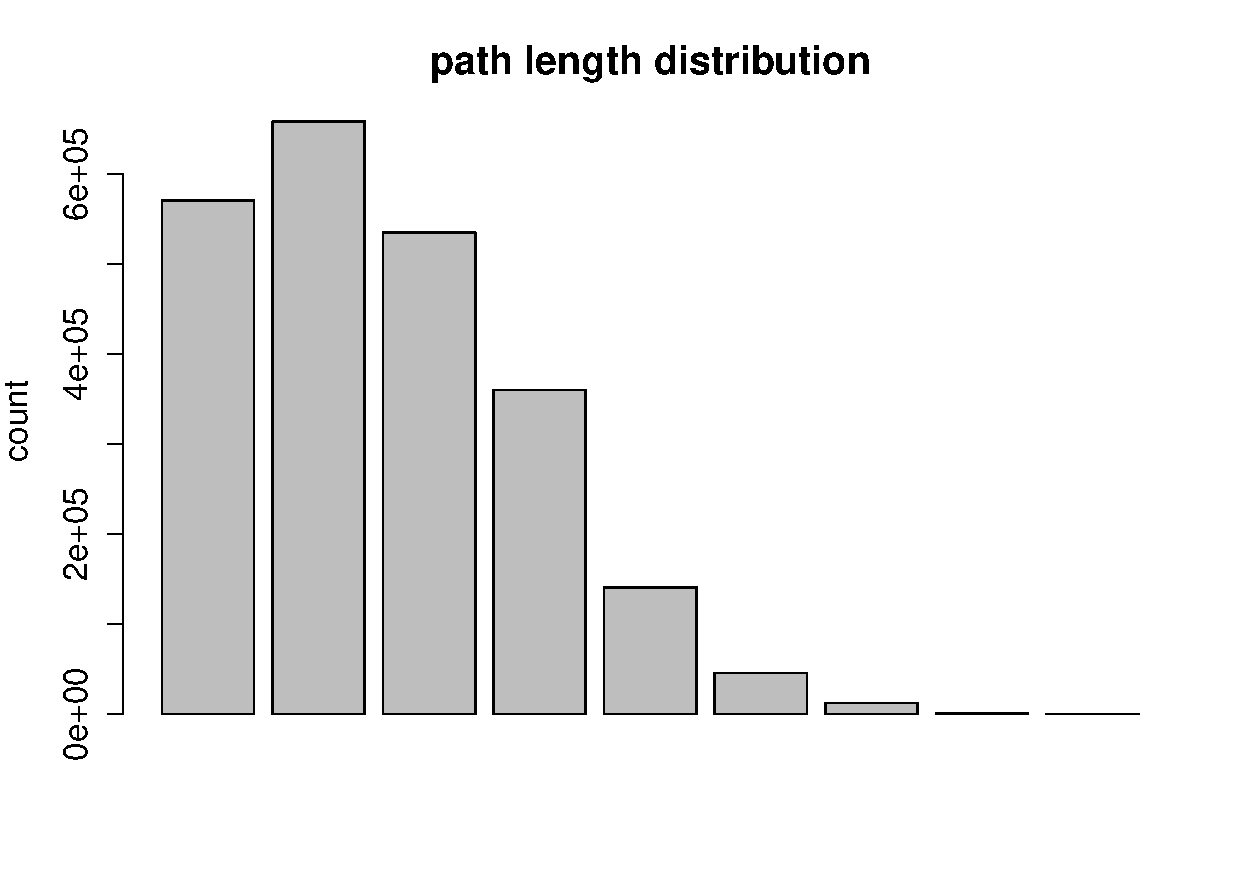
\includegraphics[width=0.5\textwidth]{figures/pathlength}
}


\jframe{Cliques(citation)}{

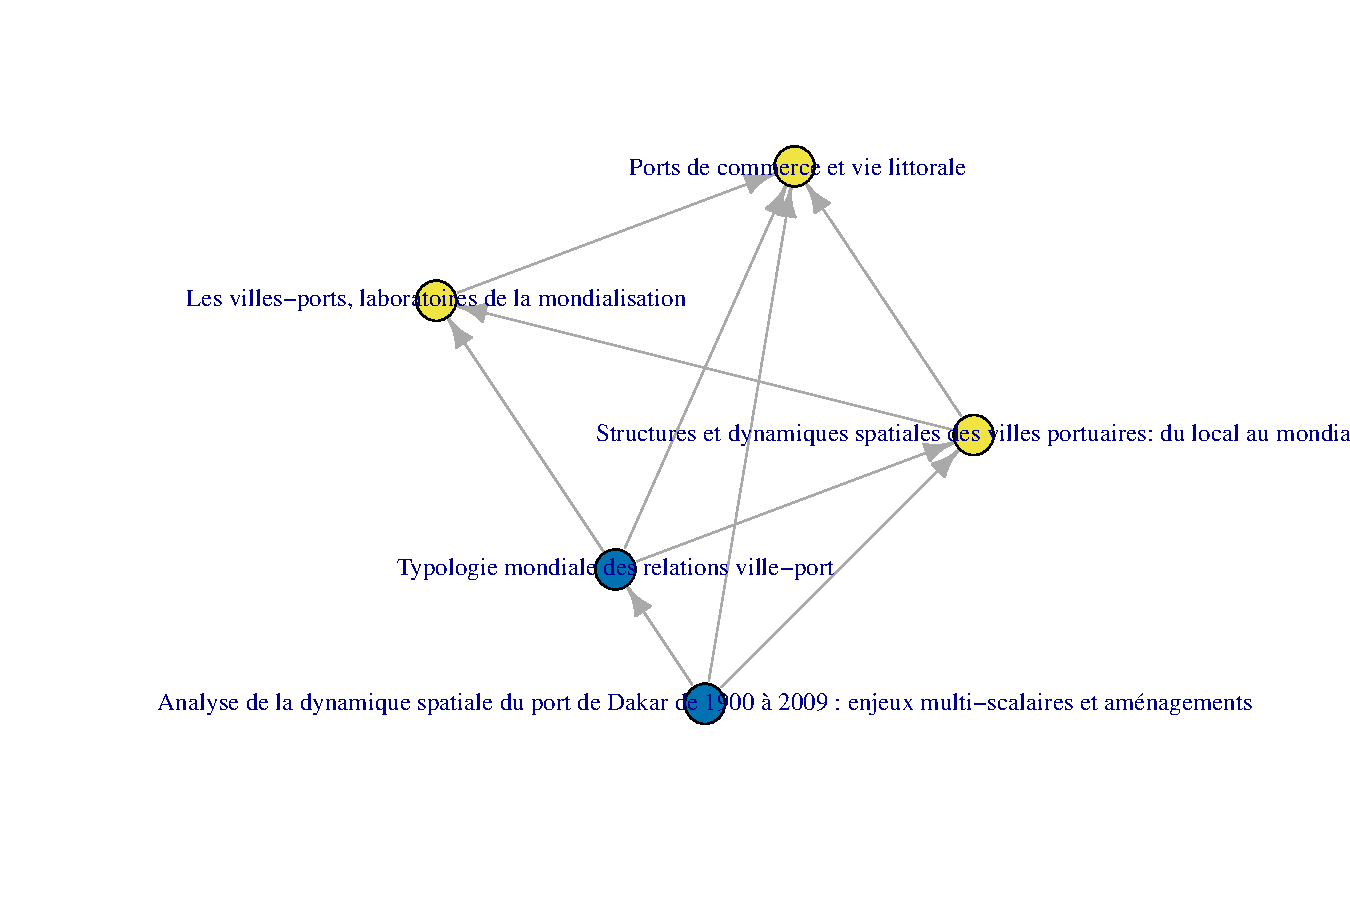
\includegraphics[height=\textheight]{figures/cybclic_2cyb_12817}

}





\jframe{Estimation de la pertinence}{
Estimation exacte de la pertinence via la repartition statistique des co-occurrences (score de $\chi^2$) : \textit{termhood} d{\'e}finie, avec $M_{ij}$ nombre d'articles où $i$ et $j$ apparaissent simultanément,
\[
t_i = \sum_{j\neq i}\frac{\left( M_{ij} - \sum_{k}M_{ik} \sum_{k} M_{jk}\right)^2}{\sum_{k}M_{ik} \sum_{k} M_{jk}}
\]


en $\Theta (\sum_i N_i^2)$ ($N_i$ taille des r{\'e}sum{\'e}s) : difficile sur un corpus o{\`u} $\sum_i N_i^2 \simeq N <N_i>^2 \simeq 8\cdot 10^7$

}











%%%%%%%%%%%%%%%%%%%%%%%%%%%%%%%%
\begin{frame}[allowframebreaks]
\frametitle{References}
\bibliographystyle{apalike}
\bibliography{/Users/Juste/Documents/ComplexSystems/CityNetwork/Biblio/Bibtex/CityNetwork,/Users/Juste/Documents/ComplexSystems/CityNetwork/Docs/Papers/Cybergeo/Biblio/cybergeo,biblio}
\end{frame}
%%%%%%%%%%%%%%%%%%%%%%%%%%%%%%%%







\end{document}
